\documentclass[usenatbib]{mn2e}
\usepackage{amsmath} 
\usepackage{amssymb} 
\usepackage{graphics}
\usepackage{graphicx}
\usepackage{epsfig}  
\def\be{\begin{equation}}
\def\ee{\end{equation}}
\def\ba{\begin{eqnarray}}
\def\ea{\end{eqnarray}}

\newcommand{\documentname}{paper~}
\newcommand{\match}{{\tt match}~}
\newcommand{\apj}{ApJ}  
\newcommand{\apjs}{ApJS}  
\newcommand{\apjl}{ApJL}  
\newcommand{\aj}{AJ}  
\newcommand{\mnras}{MNRAS}  
\newcommand{\mnrassub}{MNRAS accepted}  
\newcommand{\aap}{A\&A}  
\newcommand{\aaps}{A\&AS}  
\newcommand{\araa}{ARA\&A}  
\newcommand{\nat}{Nature}  
\newcommand{\physrep}{PhR}
\newcommand{\pasp}{PASP}    
\newcommand{\pasj}{PASJ}    

\newcommand{\kms}{\,km~s$^{-1}$}
\def\squig{\sim\!\!}
\newcommand{\LCDM}{$\Lambda$CDM~}
\newcommand{\beq}{\begin{eqnarray}}  
\newcommand{\eeq}{\end{eqnarray}}   
\newcommand{\zz}{$z\sim 3$} 
\newcommand{\avg}[1]{\langle{#1}\rangle}  
\newcommand{\ly}{{\ifmmode{{\rm Ly}\alpha}\else{Ly$\alpha$~}\fi}}
\newcommand{\hMpc}{{\ifmmode{h^{-1}{\rm Mpc}}\else{$h^{-1}$Mpc }\fi}}  
\newcommand{\hGpc}{{\ifmmode{h^{-1}{\rm Gpc}}\else{$h^{-1}$Gpc }\fi}}  
\newcommand{\hmpc}{{\ifmmode{h^{-1}{\rm Mpc}}\else{$h^{-1}$Mpc }\fi}}  
\newcommand{\hkpc}{{\ifmmode{h^{-1}{\rm kpc}}\else{$h^{-1}$kpc }\fi}}  
\newcommand{\hMsun}{{\ifmmode{h^{-1}{\rm
        {M_{\odot}}}}\else{$h^{-1}{\rm{M_{\odot}}}$}\fi}}   
\newcommand{\hmsun}{{\ifmmode{h^{-1}{\rm
        {M_{\odot}}}}\else{$h^{-1}{\rm{M_{\odot}}}$}\fi}}   
\newcommand{\Msun}{{\ifmmode{{\rm {M_{\odot}}}}\else{${\rm{M_{\odot}}}$}\fi}}  
\newcommand{\msun}{{\ifmmode{{\rm {M_{\odot}}}}\else{${\rm{M_{\odot}}}$}\fi}}  
\newcommand{\clara}{{\texttt{CLARA}}~}
\newcommand{\rand}{{\ifmmode{{\mathcal{R}}}\else{${\mathcal{R}}$ }\fi}}  
\newcommand{\Lsun}{\mbox{\,$L_{\odot}$}}
\newcommand{\like}{\mathscr{L}}
\newcommand{\bftheta}{\mathbf{\Theta}}
\newcommand{\degree}{\ensuremath{^\circ}}
\def\spose#1{\hbox to 0pt{#1\hss}}
\def\simlt{\mathrel{\spose{\lower 3pt\hbox{$\mathchar"218$}}
     \raise 2.0pt\hbox{$\mathchar"13C$}}}
\def\simgt{\mathrel{\spose{\lower 3pt\hbox{$\mathchar"218$}}
     \raise 2.0pt\hbox{$\mathchar"13E$}}}
\font\smcap=cmcsc10

\begin{document}

\title[Halo mass and occupation fraction of LAEs at$z=3.1$]{Mass and
  occupation fraction of dark matter halos hosting Lyman-$\alpha$
  emitters at $z\sim 3$}      
\author[~J.~E. Forero-Romero and ~J.~E. Mejia-Restreo]{
\parbox[t]{\textwidth}{\raggedright 
  Jaime E. Forero-Romero$^{1}$ and
  Julian E. Mej\'ia-Restrepo$^{2}$ 
}
\vspace*{6pt}\\
$^{1}$ Departamento de F\'{i}sica, Universidad de los Andes, Cra. 1
No. 18A-10, Edificio Ip, Bogot\'a, Colombia \\
$^{2}$ Departamento de Astronom\'{i}a, Universidad de Chile, Camino el
Observatorio 1515, Santiago, Chile} 

\maketitle

\begin{abstract}
%
We derive constraints on the mass and occupation fraction of dark
matter halos hosting \ly Emitting galaxies (LAEs) at a redshift of
$z=3.1$ by matching the number density and the angular
correlation function between mock and observed fields. We explicitly
take into account the cosmic variance on the typical observed field
size by constructing mock fields from a large cosmological N-body
simulation matching the geometries of observed fields. To populate the
halos in the simulation we use a model where a dark matter halo with
mass in the range $M_{\rm min}<M_{\rm h}<M_{\rm max}$ can only host
one detectable LAE with a probability $f_{\rm occ}$. The main motivation to
build such a model is to avoid the large uncertainties in the estimation of
\ly luminosities. We find that the clustering and number density information are
insufficient to impose a tight constraint on the {\bf occupation} fraction. On
the other hand the minimum mass and maximum mass are tightly
constrained to be $M_{\rm max}<10^{12}$\hMsun and
$10^{10}\hMsun\leq M_{\rm min}\leq 10^{11.5}\hMsun$.  We also find
that all models have a narrow mass range $\Delta M \equiv
\log_{10}M_{\rm max} - \log_{10} M_{\rm min}$ smaller than $1.0$ dex,
with the vast majority in the range $\Delta M<0.5$ dex. Already
published constraints on the mass range and occupation fraction are a sub-set of
the models we report in this \documentname. Our results present an
inconclusive response as to which is the occupation fraction for LAEs
at $z=3.1$. A precise answer requires robust physical models for the
connection between dark matter, star formation and the escape of \ly
radiation. That kind of modelling should also be able to provide a
plausible explanation for the narrow range in mass $\Delta M<1.0$ dex
derived here for the halos hosting LAEs at $z=3.1$.   

\end{abstract}

\begin{keywords}
{cosmology: theory – cosmology: large-scale structure of universe –
  galaxies: formation – galaxies: high-redshift – galaxies: statistics
  – galaxy: haloes} 
\end{keywords}


\section{Introduction}

Lyman-$\alpha$ emitting galaxies (LAEs) have become in the last decade
a  central topic in studies of structure formation in the Universe. They 
are helpful in a diverse range of fields. LAEs can be used as probes
of reionization \citep{Dijkstra11}, tracers of large scale structure
\citep{Koehler2007},  signposts for low metallicity stellar
populations, markers of the galaxy formation process at high redshift
\citep{Dayal2009,ForeroRomero2012} and tracers of active star formation
\citep{Guaita2013} 

At the same time, theoretical and observational developments have
contributed to the emergence of a paradigm to describe structure
formation in a cosmological context. In this context it is considered
that the dominant matter content of the Universe is to be found in dark
matter (DM), whereby each galaxy is hosted by larger dark matter structure
known as a halo. \citep{Peebles1980,SpringelNature05}.

Most models of galaxy formation find that halo mass can be
used to predict galaxy properties such as the stellar mass and
star formation rate \citep{Behroozi2013a}. Processes that regulate the
star formation cycle are also though to be strongly dependent on its
halo mass.  For these reasons, finding the typical dark matter halo mass
hosting LAEs represents a significant step forward to understand the
nature of this galaxy population in the context of Lambda Cold Dark
Matter ($\Lambda$CDM) paradigm.    

Some theoretical approaches to this problem have been based on
ab-initio approach. Starting from the DM halo population, the
corresponding intrinsic star formation properties are inferred
together with other statistics such as the luminosity function, the
correlation function and the equivalent width distributions. Such
modelling has been implemented from analytic considerations,
semi-analytic models \citep{Garel2012, Orsi2012}and  full N-body
hydrodynamical simulations \citep{Laursen2007, Dayal2009,
  ForeroRomero2011, Yajima2012, Soler2012}.   

In addition to the uncertainties in the astrophysical processes
describing star formation in galactic populations,the calculation
of the fraction of \ly photons that escape the galaxy to the observer
is another debated step. Given the resonant nature of the \ly line,
the radiative transfer of \ly is sensitive to the density,
temperature, topology and kinematics of the neutral Hydrogen in the
interstellar medium
(ISM). This problem can be tackled with Monte Carlo simulations for the
radiative transfer, however the complexity of the relevant physical
processes makes it difficult to achieve a robust consensus on what is
the theoretical expected value for the \ly escape fraction
at high redshift
\citep{Neufeld1991,Verhamme2006,ForeroRomero2011,Dijkstra2012,Laursen2013,Orsi2012}. 

Another approach to infer the typical DM halo mass of halos hosting
LAEs is based on the clustering information. This uses the fact that in cold
dark matter cosmologies the spatial clustering of galaxies on large
scales is entirely dictated by the halo distribution
\citep{Colberg00}, which in turn has a strong dependence on halo
mass. Using measurements of the angular correlation function of LAEs,
observers have put constraints on the typical mass and occupation
fraction of the putative halos hosting these galaxies
\citep{Hayashino2004,Gawiser07,Nilsson2007,Ouchi2010}. In this
studies the observations were done on single fields of $\sim 1$
deg$^{2}$ and the conclusions derived on the halo host mass from
clustering information do not delve to deeply into the impact of
cosmic variance.

Recently \cite{Yamada2012} observed a wide area a bit more than ten
times the sky area covered so far by individual campaigns. The
observations were done with the same instrument and same criteria to
reduce the observational data and produce LAE catalogs. This large
data-set allows us to make the first study on the expected cosmic
variance effects in LAEs at $z=3.1$ and its impact on the
determination of the halo mass and occupation fraction. 


In this \documentname we implement a method to populate the DM halos
in cosmological simulations with LAEs that bypasses all the
uncertainty involved in the estimation of star formation rates and \ly escape
fraction. The model only considers whether a DM can host a
detectable LAE or not without predicting a \ly  luminosity. Once the
mock catalogs are constructed  we proceed with a direct comparison
against the statistics derived from observations. This allows us 
to find the preferred mass range of DM halos hosting these galaxies
and its occupation fraction.


This \documentname is structured as follows. In the next section we present
the simulation and model used to produce the mock catalogs and the criteria
we use to compare them against observations. In \S \ref{sec:results} we
present the main results for the halo mass and occupation fraction. We
continue with a discussion of these results under the light of other
observational and theoretical results. Finally, we present our
conclusions in \S \ref{sec:conclusions}. 

Throughout this \documentname we assume a $\Lambda$CDM cosmology with the
following values for the cosmological parameters, $\Omega_{m}=0.27$,
$\Omega_{\Lambda}=0.73$ and $h=0.70$, corresponding to the matter
density, vacuum density and the Hubble constant in units of 100 km
s$^{-1}$ Mpc$^{-1}$. 

\section{Methodology}


Our method is based on the comparison of observations and mock
catalogs. We use two different kinds of statistics to perform the
comparison: (i) the distribution of the surface number density
across fields and (ii) the angular correlation function measured in
some fields.

In the next subsections we describe in detail the four key
elements of this work-flow. First, we present the observations we take
as a benchmark. Second, we describe the main characteristics of the
N-body simulation and the halo catalogs we use. Third, we recount the
important parameters of the simplified model that we use to populate
the halo catalogs with LAEs. Finally we describe some of the
statistical tests we adopt to compare observations and mocks.

\subsection{Observational constraints}

The first observational constraint we use in this paper is the LAE number
density information at $z=3.1$ obtained by the panoramic narrow-band
survey presented by \cite{Yamada2012} from a survey
conducted with the Subaru 8.2m telescope and the Subaru Prime Focus Camera,
which has a field of view covering $34\times 27$ arc-min, corresponding to a
comoving scale of $46\times35$ Mpc $h^{-1}$ at $z=3.09$.  The narrow
band filter used in the survey is centered at $4977$ \AA~with  $77$ \AA~width,
corresponding to the redshift range $z=3.062$-$3.125$ and $41$ \hMpc
comoving scale for the detection of the Lyman-$\alpha$ line centered
at $z=3.09$. The authors reported a total  $2161$  LAEs with an
observed equivalent width, in the observer frame, larger than $190$
\AA~over a total survey area of $2.42$ deg$^{2}$ that includes 12
sub-fields,  this corresponds to average surface number density of
$0.20\pm 0.01$ arcmin$^{-2}$.    

The survey covered four independent fields. The first is the SSA22
field of $1.38$ deg$^2$ with $1394$ detected LAEs (7 sub-fields), this
field has been known to harbor a region with a large density excess of
galaxies. The second observed region is composed by the fields Subaru/{\it
  XMM-Newton} Deep Survey (SXDS)-North, -Center and -South, with a
total of $0.58$ deg$^2$ and $386$ LAEs (3 sub-fields). The third and
fourth fields are the Subaru Deep Field (SDF) with $0.22$ deg$^2$ and
$196$ LAEs (1 sub-field), and the field around the Great Observatory
Optical Deep Survey  (GOODS-N) with $0.24$ deg$^2$ and $185$ LAEs (1
sub-field).  

There is abundant observational work done on LAEs at redshift $z=3.1$
\citep{Kudritzki2000,Matsuda2005,Gawiser2007,Nilsson2007,Ouchi2008}.
However, we decide to focus on the data from \cite{Yamada2012} because
it has the largest covered area with homogeneous instrumentation
conditions (telescope, narrow band filter), data reduction pipeline
and conditions to construct the LAE catalog. This ensures that the
number density variations among fields are \emph{not} due to different
observational conditions or criteria to construct the catalogs.

The second constraint is the angular correlation function
(ACF). {\bf \cite{Yamada2012} does not report an ACF measurement}. Instead
we use the results by \cite{Hayashino2004} and
\cite{Ouchi2008,Ouchi2010}. \cite{Hayashino2004} observed in the
densest field of SSA22 while \cite{Ouchi2008} observed a 1 deg$^2$
over the SXDS field, which is twice as large as the SXDS region
observed by \cite{Yamada2012}.

There are some differences between these observations and those by
\cite{Yamada2012}. The details in the color selection, corresponding
limiting luminosities and EW thresholds are different in these
references. Nevertheless we use the ACF from these observations as
additional constraints in spite of the fact that the first selected
models are based only on the surface density statistics by \cite{Yamada2012}.  

{\bf The LAEs number density inferred by \cite{Hayashino2004} is
  $0.37$ arcmin$^{-2}$, which is $15\%$ lower than the new measurement
by \cite{Yamada2012}. In the case of \cite{Ouchi2008} the number
density is $0.10$ arcmin$^{-2}$, which is $\sim 50\%$ than the value
inferred by \cite{Yamada2012} for a portion of the same region.}

\subsection{The adequacy of using SSA22 as an observational test}

{\bf The field centered on SSA22 has been known to harbor a 
  galaxy overdensity. Measurements of Lyman Break Galaxies show that
  the densest sub-field presents an overdensity 6 times the one present in a
  blank field \cite{XXX}. Using the data of \cite{Yamada2012}, we
  compute that for LAEs the whole region is only 1.4 times more dense than
  the blank fields of SXDS, SDF and GOODS-N. The densest sub-field
  in SSA22 is only 2 times denser than the average of the blank
  fields.}

{\bf This shows that the bias factor of LBGs is higher
  than LAEs. In a LCDM cosmology this implies that LAEs are, on average,
  hosted by halos less massive than those hosting LBGs. The
  interpretation of how rare is this subfield in terms of the number
  densities of dark matter halos has to assume a defined model for
  galaxy formation[...]} 



{\bf Excluding the densest region in the SSA222, all the fields have a
similar number densisty as the blank fields and cannot be considered
as rare. The left panel in Figure \ref{fig:halos} shows the integrated
distritbution of LAEs number density in all the fields reported in
\cite{Yamada2012}. 


From this figure it is clear that the highest density
sub-fields is the only outlier in the distribution. Therefore, using
as a benchmark the number density distribution that includes the
sub-fields in the SSA22 region does not impose a strong bias to select
very rare regions in a cosmological simulation. However, on has to
keep in mind that only very rarely the full number density distribution from a
simulation will include a very dense field as an outlier. We will not
require the presence of such field to judge a mock distribution as
successful. [...]} 


\subsection{Simulation and halo catalogs}

The Bolshoi simulation \citep{Bolshoi} we use in this paper was
performed in a cubic volume of 250 $h^{-1}$ Mpc on a side. The
dark matter distribution is sampled using $2048^{3}$ particles, which
translates into a particle mass of $m_{\rm   p}=1.35\times 10^{8}$
$h^{-1}$ M$_{\odot}$.  The cosmological parameters are consistent with
a WMAP5 and WMAP7 data with a matter density $\Omega_{\rm m} = 0.27$,
cosmological constant $\Omega_{\Lambda}=0.73$, dimensionless Hubble constant
$h=0.70$, slope of the power spectrum $n=0.95$ and normalization of the
power spectrum$\sigma_{8}=0.82$ \citep{Komatsu2009,Jarosik2011}.  

We use halo catalogs constructed with a Friend-of-Friends (FOF)
algorithm with a linking length of 0.17 times the inter-particle
distance. The catalogs were obtained from the publicly available
Multidark database \footnote{{\tt
    http://www.multidark.org/MultiDark/}}
\citep{MultiDark}. For each halo in the box we store its
comoving position in the box (3-D coordinates) and FOF mass. We focus our work
on halos more massive than $1\times 10^{10}$\hMsun that are resolved
with at least $70$ particles, the reasons for this choice are
explained in the next sub-section.  


\subsection{A model to populate halos with LAEs}
\label{subsec:mocks}



\begin{figure*}
\begin{center}
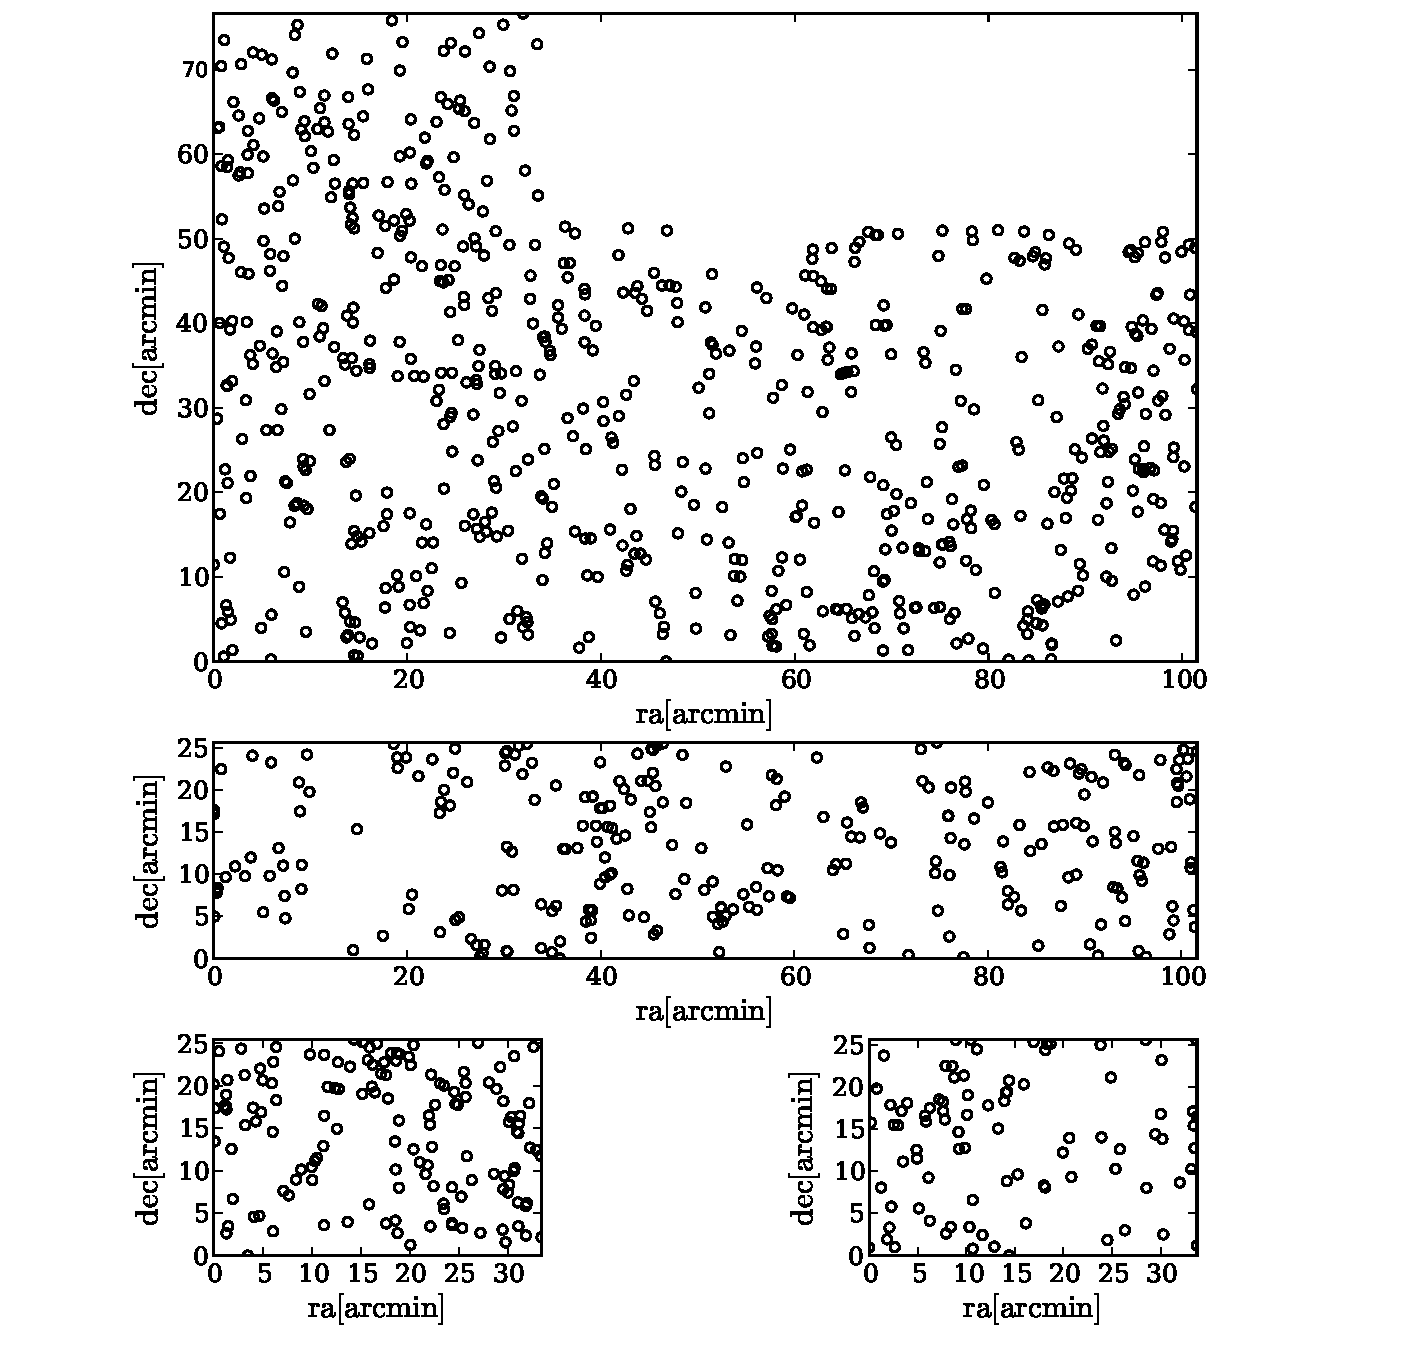
\includegraphics[width=0.8\linewidth,angle=0]{Figure0.pdf}
\caption{ \label{fig:distros} Spatial distribution of a LAEs mock
  survey for a model with parameters $\log_{10}M_{\rm min}=10.4$, $\log_{10}M_{\rm
    max}=10.5$ and $f_{\rm occ}=0.1$ for the {\texttt{match}}
  method. The larger panel shows $7$ mock
  fields together mimicking the SSA22 region. The intermediate panel
  shows $3$ mock fields corresponding to the SXDS region. The lower
  panels represent the SDF and GOODS-North fields. The same model has
  another 14 associated mock surveys build from different regions in
  the simulation, but constructed following the same pattern in the
  {\texttt{match}} method.}
\end{center} 
\end{figure*}



We assume that a dark matter halo can only host one
detectable LAE at most.  There are three parameters that
decide whether a halo host a LAE: the lower and upper bounds for the
mass range, $M_{\rm min}< M_{\rm h} < M_{\rm max}$, where LAEs reside and the fraction $f_{\rm occ}$ of such halos that host a detectable LAE. The reader
must keep in mind that the physical interpretation of the occupation
fraction $f_{\rm occ}$ convolves two phenomena: the actual presence of a star
forming galaxy in a halo and its detectability as a LAE.  We do not
perform a explicit modeling for LAE detectability. Our model does not
assign a luminosity or escape fraction to each LAE.  We are only
interested in constraining the halo mass range hosting detectable LAEs
under the conditions defined by \cite{Yamada2012}.  


In what follows we note by the letter ${\mathcal M}$ a model
defined by a particular choice of the three scalar parameters $M_{\rm
  min}$, $M_{\rm  max}$ and $f_{\rm occ}$. For each model ${\mathcal
  M}$ we create a set of mock fields from disjoint volumes in the
simulation. Each volume has the same geometry probed by Suprime-CAM
and the narrow band filter, namely rectangular cuboids of dimensions
$46\times 35\times 41$ $h^{-3}$ Mpc$^{3}$ where the last dimension goes
in the redshift direction. This corresponds to a total area of $880$
arcmin$^{2}$ in each mock field. We construct a total $5\times 7
\times 6=210$ of such volumes from a snapshot in the Bolshoi
simulation. In each mock field a LAE is assigned to the position of a
dark matter halo if the halo mass is in the range allowed by the model
$M_{\rm min}<M_{\rm h}<M_{\rm max}$ and a random variable taken from
an homogeneous distribution $0\leq \xi<1$ is smaller than the occupation
fraction $\xi<f_{\rm occ}$.

Next we construct mock surveys by making groups of $12$ mock fields
out of the $210$ available volumes. In total $15$ mock surveys are
constructed for each model $\mathcal{M}$. The grouping of the $12$
mock fields into a mock catalog is done in two different ways. The
first is called {\texttt{match}}, it follows the clustering of the
observational fields. From the $12$ mock fields, $7$ are constructed
from contiguous fields in the simulation to mimic the SSA22 region,
$3$ are also contiguous between them but not to the first $7$ fields
to mimic the SXDS fields and finally $2$ non-contiguous fields to
imitate the SDF and GOODS-North field.   The second way to group the
mock fields is called {\texttt{random}}, whereby all the $12$ fields
are selected in such a way as to avoid that any two volumes are
contiguous. In this \documentname we only report the results obtained
by the {\texttt{match}} method and mention explicitly differences
observed with the {\texttt{random}} selection. 


Figure \ref{fig:distros} shows the spatial distribution for one mock
survey constructed using the {\texttt{match}} method. Each field
corresponds to one of the observational fields. The model parameters
to build it are $M_{\rm min}=10^{10.4}$\hMsun, $M_{\rm
  max}=10^{0.5}$\hMsun and $f_{\rm occ}=0.1$. It is only one out of
the $15$ different mock surveys that are constructed for each
model. We note that we use $15\times 12=180$ mock fields out of the
total of $210$ available sub-volumes. The reason is that the {\texttt{match}}
method imposes constraints on the way the $7$ fields mimicking the
SSA22 can be distributed. This restriction makes unable some of the
sub-volumes in the box. We decide to keep the number of mock surveys
fixed to $15$ also for the {\texttt{random}} method in order to allow a
fair comparison between the two methods.




\subsection{Exploring and selecting good models}


\begin{figure*}
\begin{center}
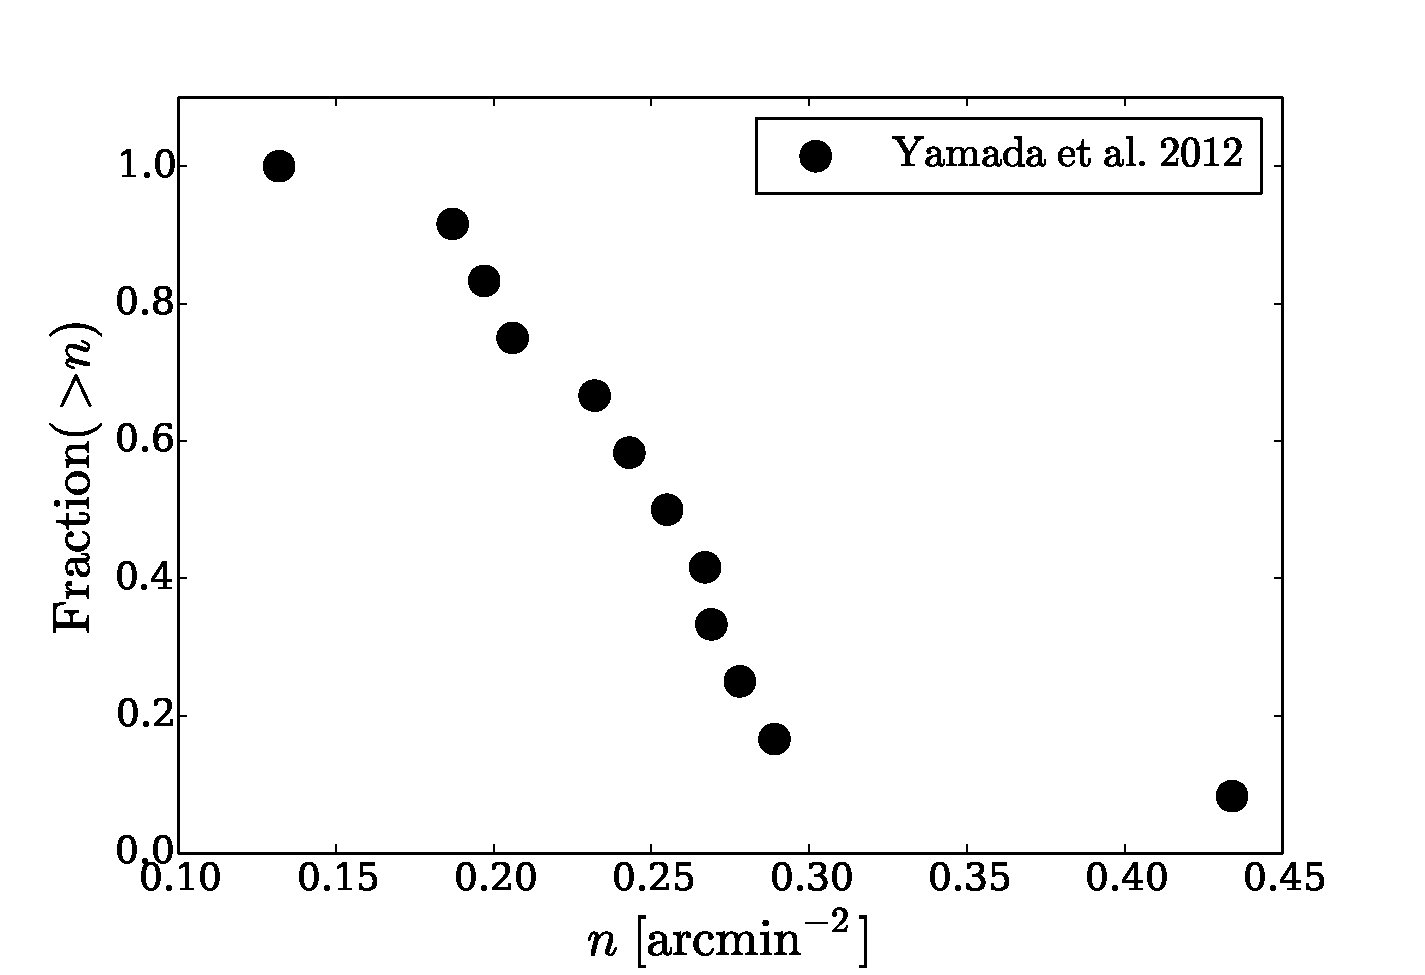
\includegraphics[width=0.45\linewidth,angle=0]{Fig1b.pdf}
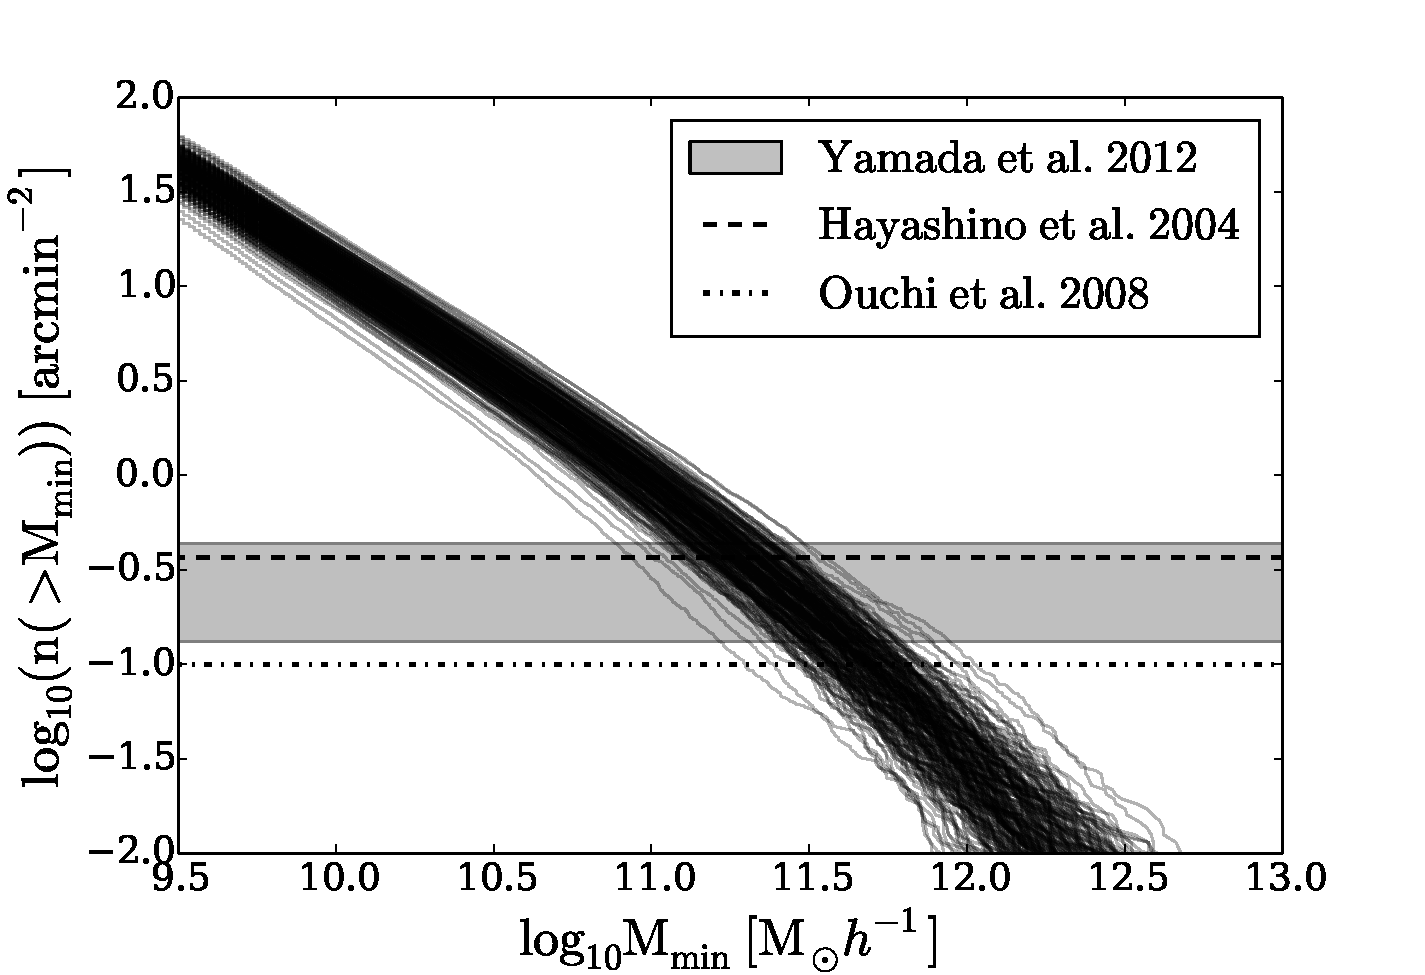
\includegraphics[width=0.45\linewidth,angle=0]{Fig1.pdf}
\caption{ \label{fig:halos} Left panel. Distribution of LAE number
  densities in all the fields observed by \citet{Yamada2012}. The
  point with the highest surface density corresponds to the densest
  sub-field in the SSA22 field. Right panel. Surface density of dark 
  matter halos as a function of a minimum halo mass to count the
  total number of elements in a volume. Each line represents one of the
  $210$ volumes of dimensions $46\times 35\times 41$ $h^{-3}$ Mpc$^{3}$
  in the Bolshoi simulation. The horizontal gray band represents the
  range of surface densities observed for LAEs at $z=3.1$ as reported
  by \citep{Yamada2012}.}
\end{center} 
\end{figure*}


We make a thorough exploration of the parameter space for the models
${\mathcal M}$ where $\log_{10} M_{\rm min}$ takes $30$ values from $10.0$ up
to $12.9$ with an even spacing of $0.1$ dex. $\log_{10} M_{\rm max}$
takes values in the same range as $\log_{10}M_{\rm min}$ only with a
displacement of $0.1$ dex in the whole range. The occupation fraction
$f_{\rm occ}$ takes $10$ different values from $0.1$ to $1$ regularly
spaced by $0.1$. In total the number of different models ${\mathcal
  M}$ that are explored is $30 \times 30 \times 10 = 9000$. 


The lower limit for the parameter $M_{\rm min}$ is set by the minimum
occupation fraction we are able to consider. At $M_{\rm
  min}=10^{10}$\hMsun the halo number density is already $\sim 10$
times higher than the observational constraints for LAEs. This means
that models in that mass range and an occupation fraction $f_{\rm
  occ}=0.1$ have the possibility to be compatible with observations. Lower
values for $M_{\rm min}$ require $f_{\rm occ}<0.1$, which are not
considered in this \documentname. 

For each mock survey generated in a given model ${\mathcal M}$ we
compute the surface density in the $12$ mock fields. We perform a
Kolmogorov-Smirnov (KS) to compare this mock data against the $12$
observational values. From this test we obtain a value $0<P<1$ to
reject the null hypothesis, namely that two data sets come from the
same distribution. In this paper we consider that for values $P>0.05$
the two distributions can be thought as coming from the same
distribution.

We begin by considering that  a model ${\mathcal M}$ that has at least
one mock survey (out of 15) consistent with the observed
distribution of LAE number densities has viable parameters that
deserve to be considered for further analysis. Later on we impose
harder constraints to reduce the number of models by asking that all
the 15 mocks to be consistent with observations.

The second constraint  comes from the angular correlation function (ACF)
for all the models having the $15$ mock surveys consistent with
observations . The ACF is computed using 
the Landy \&  Szalay estimator \citep{Landy1993}  on two different 
fields in the mock survey. The first field is the densest to be compared
against the results of \cite{Hayashino2004}. The second field
has an average number density and is compared against \cite{Ouchi2010}.

The observed and mock ACF are fit to a power-law function:
\begin{equation}
\omega(\theta) = \left(\frac{\theta}{\theta_{0}}\right)^{-\beta}, 
\label{eq:fitting}
\end{equation}
where $\theta_0$ and $\beta$ are free parameters. The fit is done
using a least square minimization procedure. For each mock field we obtain a
covariance matrix that gives us the uncertainty in the parameters $\beta$ and
$\theta_0$. Using the $15$ mock fields in a mock survey, we compute a
mean value for the parameters and its associated uncertainty as the
quadratic average of the uncertainties in the fitting procedure. We
consider that a model is consistent with observations if the two
parameters $\beta$ and $\theta_0$ are equal within a $1$-$\sigma$
range.   



 
\section{Results}
\label{sec:results}

The main purpose of this section is to show how different
observational constraints narrow down the parameters space of allowed
models. Each sub-section presents the effect of adding new pieces of
observational or statistical evidence. 


\subsection{Dark Matter Halo Number Density}

In Figure \ref{fig:halos} we present the results for  the
integrated dark matter halo surface density as a function of the
minimum halo mass $M_{\rm min}$. Each line corresponds to one of the
210 sub-volumes in the Bolshoi simulation. The gray band indicates the
surface density values for LAEs allowed by observations
\citep{Yamada2012}. 
 
This result allows us to understand why only a specific range of
models ${\mathcal M}$ can be expected to be consistent with
observations. From Figure \ref{fig:halos} we can read that models with
a minimum mass $M_{\rm min}>10^{11.5}$\hMsun will always have a
surface number density lower than the observational constrain. This
makes impossible that models in that range can be compatible with
observations, there are simply to few halos compared to observed
LAEs. The opposite is true in models with $M_{\rm
  min}<10^{10.5}$\hMsun that have a surface number density larger
observations. In those cases the occupation fraction $f_{\rm occ}<1.0$
can be tuned in order to lower the halo number density to match
observations.  


Figure \ref{fig:halos} also illustrates the impact of cosmic
variance. At fixed mass there is an scatter of $0.3-0.6$ dex in the
number density abundance.  A consequence of this variation is that
models with the same mass range and occupation fraction can have mock
fields with number densities varying up to a factor of $\sim
2-5$. This scatter is comparable to the $0.3$ dex scatter coming from 
observations. In the same Figure \ref{fig:halos} we see that at fixed
number density, around the range allowed by observations, there is an
scatter in the masses of $0.4-0.5$ dex.  

This scatter induced by cosmic variance is naturally included in the
mock construction process. This will allows us to have a wider range
of models compatible with observations, as compared with a model that
neglects cosmic variance.


\subsection{Models consistent with the surface density distributions}

\begin{figure*}
\begin{center}
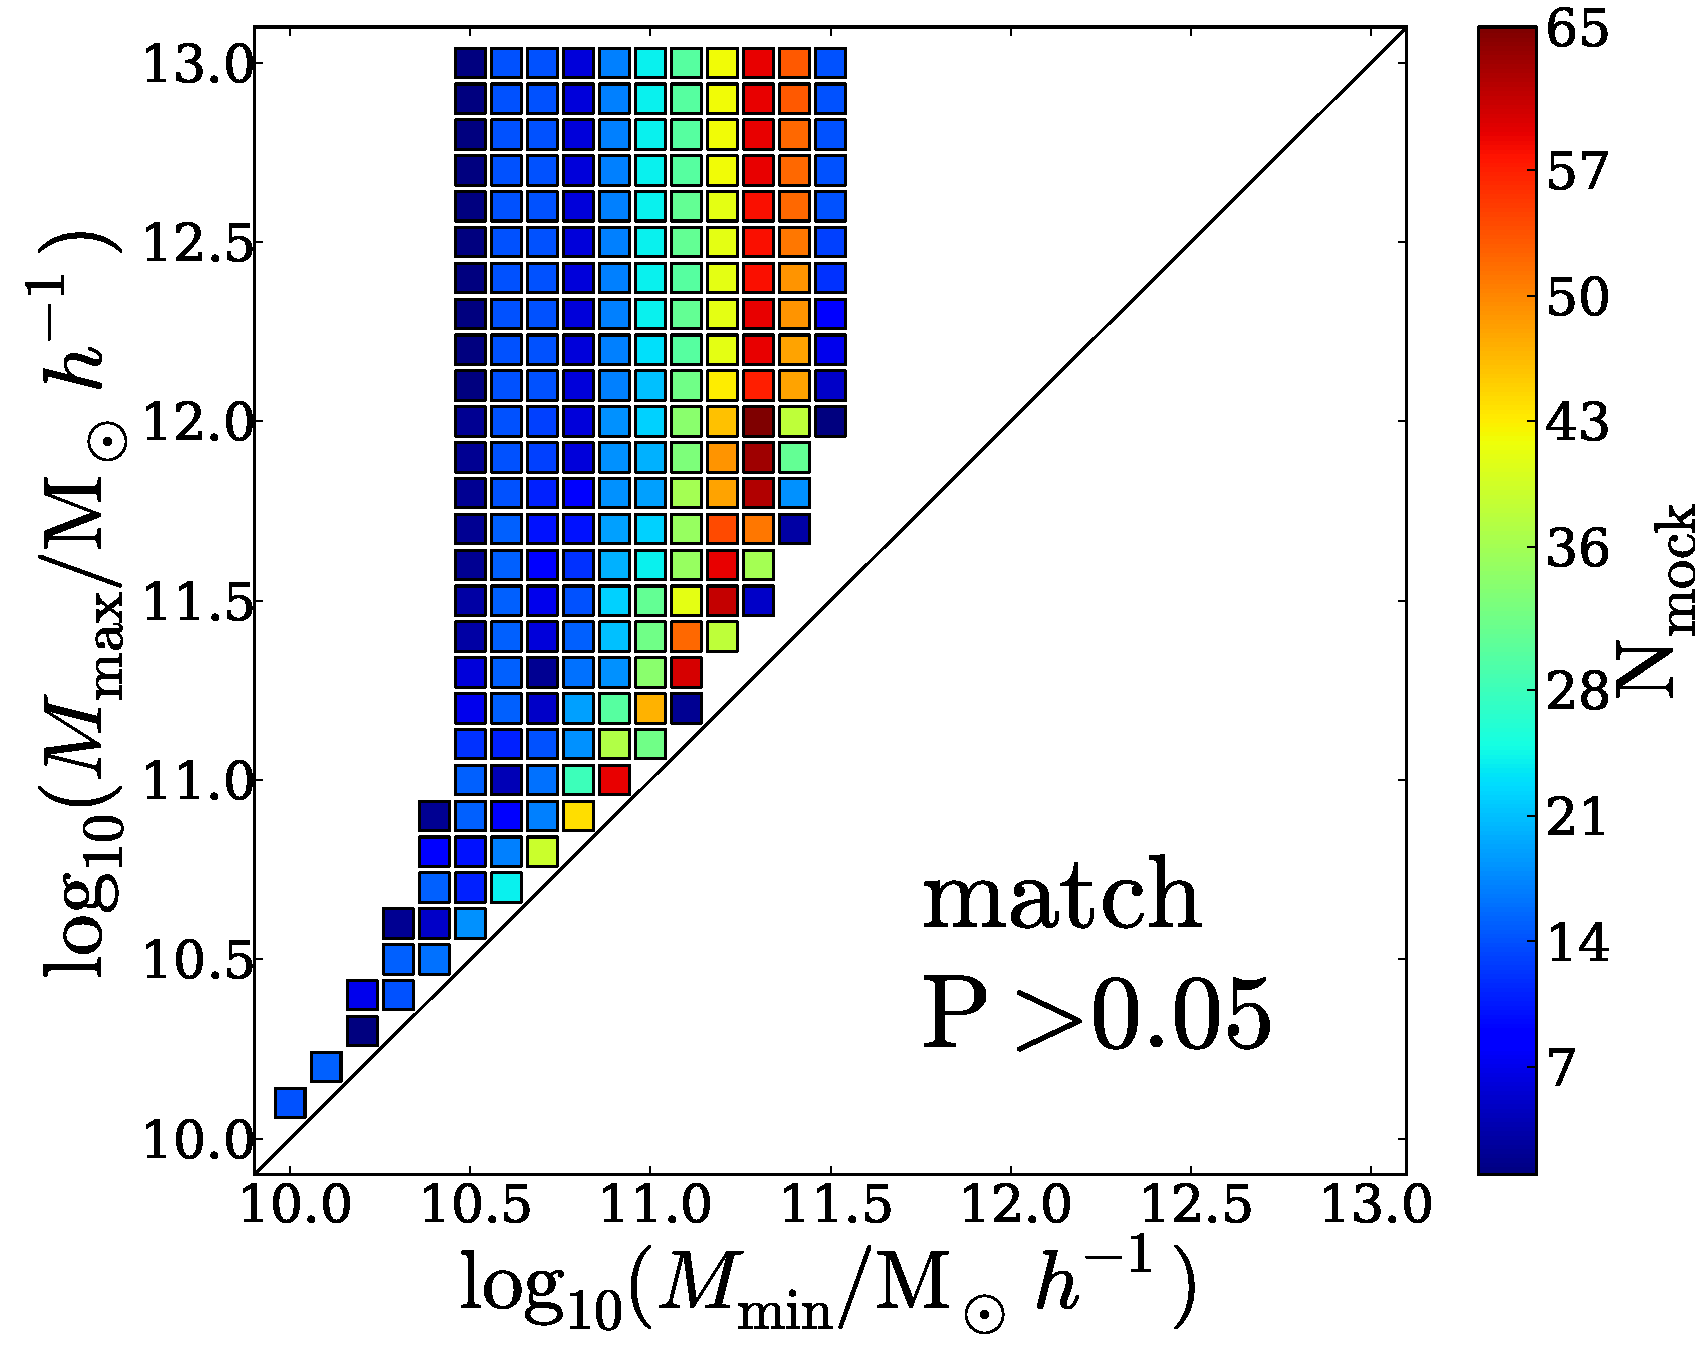
\includegraphics[width=0.46\linewidth,angle=0]{Fig2_match_P5.pdf}
\vspace{5mm}
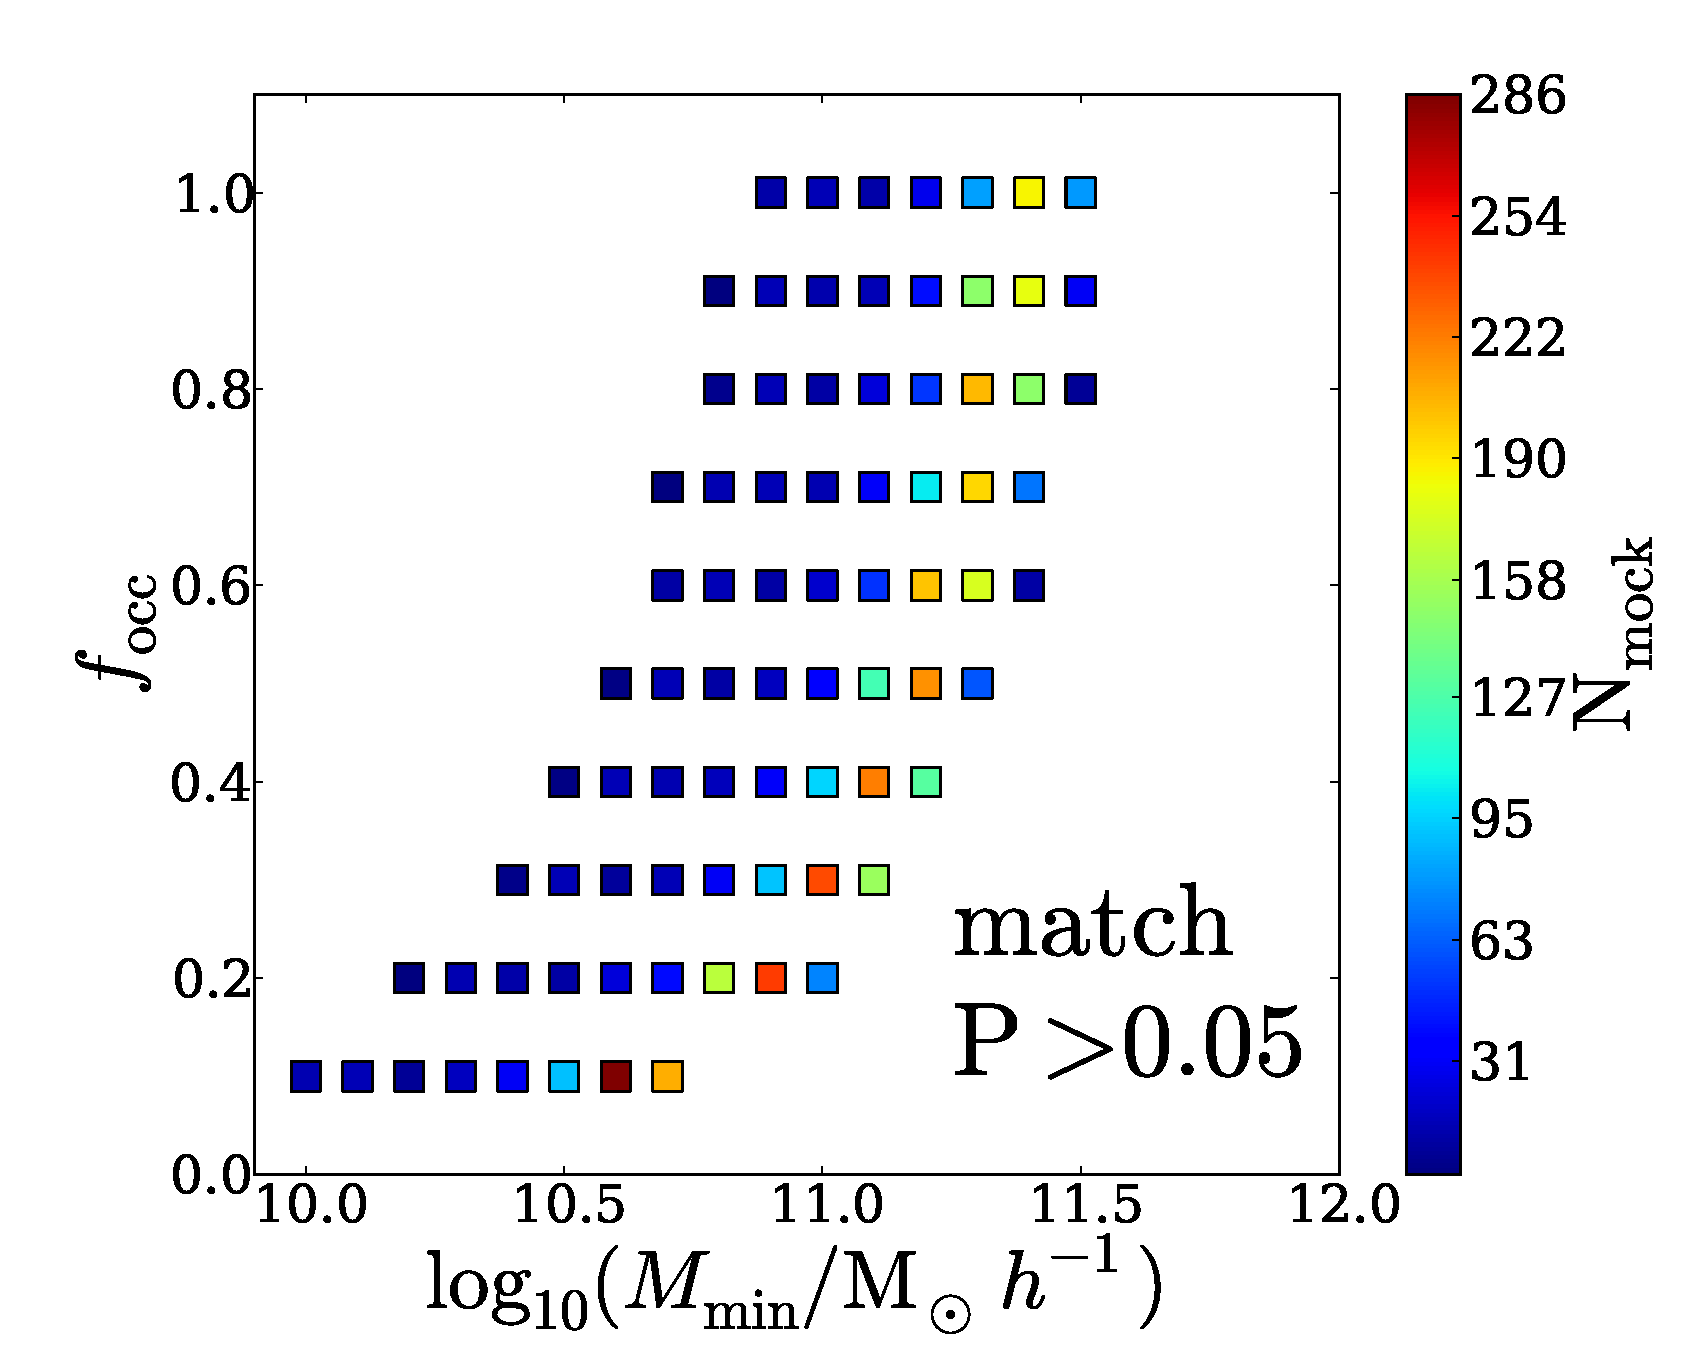
\includegraphics[width=0.49\linewidth,angle=0]{Fig3_match_P5.pdf}
\end{center} 
\caption{$M_{\rm min}$-$M_{\rm max}$ (left) and $M_{\rm    min}$-$f_{\rm
    occ}$ (right) planes for all models with  KS test values
  $P>0.05$. The color code corresponds to the number of mock surveys
  compatible with observations. Only regions of parameter  space with
  at least one consistent mock survey are  included. \label{fig:landscape}}     
\end{figure*}


Figure \ref{fig:landscape} presents regions in parameter space $M_{\rm
min}$-$M_{\rm max}$, $M_{\rm min}$-$f_{\rm occ}$ where the KS test yields
values of $P>0.05$ at least for one mock survey, which is the most
conservative assumption for agreement between a model and observations. For those models it
is not possible reject the hypothesis that the simulated and observed
data for the surface number density come from the same parent
distribution. In total, there are between $550$ to $600$ models out of
the original $9000$ models that have at least one mock survey
consistent with observations. By inspection of Figure
\ref{fig:landscape} we see that the halo number abundance is able to
constraint the minimum mass $M_{\rm min}$ to a narrow range, while
$M_{\rm max}$ and $f_{\rm occ}$ remain largely unconstrained.

In Figure \ref{fig:landscape} there are three regions of parameter
space that can be clearly distinguished. The first corresponds to
models where the minimum mass is high $M_{\rm min}>
10^{11.5}\hMsun$. None of these models is compatible with observations
as expected from the arguments presented in the previous
subsection. For these models the number density of LAEs is too low
compared to observations.

 
The second region corresponds to an intermediate range for the minimum
mass $10^{10.5}\hMsun < M_{\rm min}< 10^{11.5}\hMsun$ where,
regardless of the value of the maximum mass $M_{\rm max}$, it is
possible to tune the occupation fraction $f_{\rm occ}$ to bring some
of the mock surveys into good agreement with observations. In this
region of parameter space one can find two extreme kinds of models.
One kind where the mass interval $\Delta M\equiv \log_{10} M_{\rm max}
- \log_{10}M_{\rm  min}$ is narrow with $\Delta M<1.0$ dex, others
where the mass interval is  extended $\Delta M>1.0$ dex going up to
the maximum halo mass present in the simulation at that redshift, with
$\Delta M = 2.5$ dex in those cases.
 
The third region in parameter space corresponds to $M_{\rm
  min}<10^{10.5}\hMsun$. In this case only models with a very narrow
mass interval of at most $0.5$ dex ($M_{\rm max}<10^{11.0}\hMsun$) and low
occupation fractions $f_{\rm occ}\leq 0.3$ are allowed. 

Without any additional information our method allows us to infer that
most of the successful models are found in the second and third regions of
parameter space. This result was already expected from halo
abundance calculations shown in Figure \ref{fig:halos} and discussed
in the previous subsection. 

However, the additional information we gain with this test is the
relative abundance of models in the parameter space. Not all 
models in the second region have an equal abundance. By inspection of
Figure \ref{fig:landscape} it seems that models with $\log_{10}M_{\rm
  min}\sim 10^{11.3}$\hMsun and low occupation fraction $f_{\rm}\leq 0.3$
are preferred.  In the next sub-sections we explore in detail the
models in this region, imposing tighter constraints on the KS test
results and exploring the mocks' consistency with the angular correlation
function.  

\begin{figure}
\begin{center}
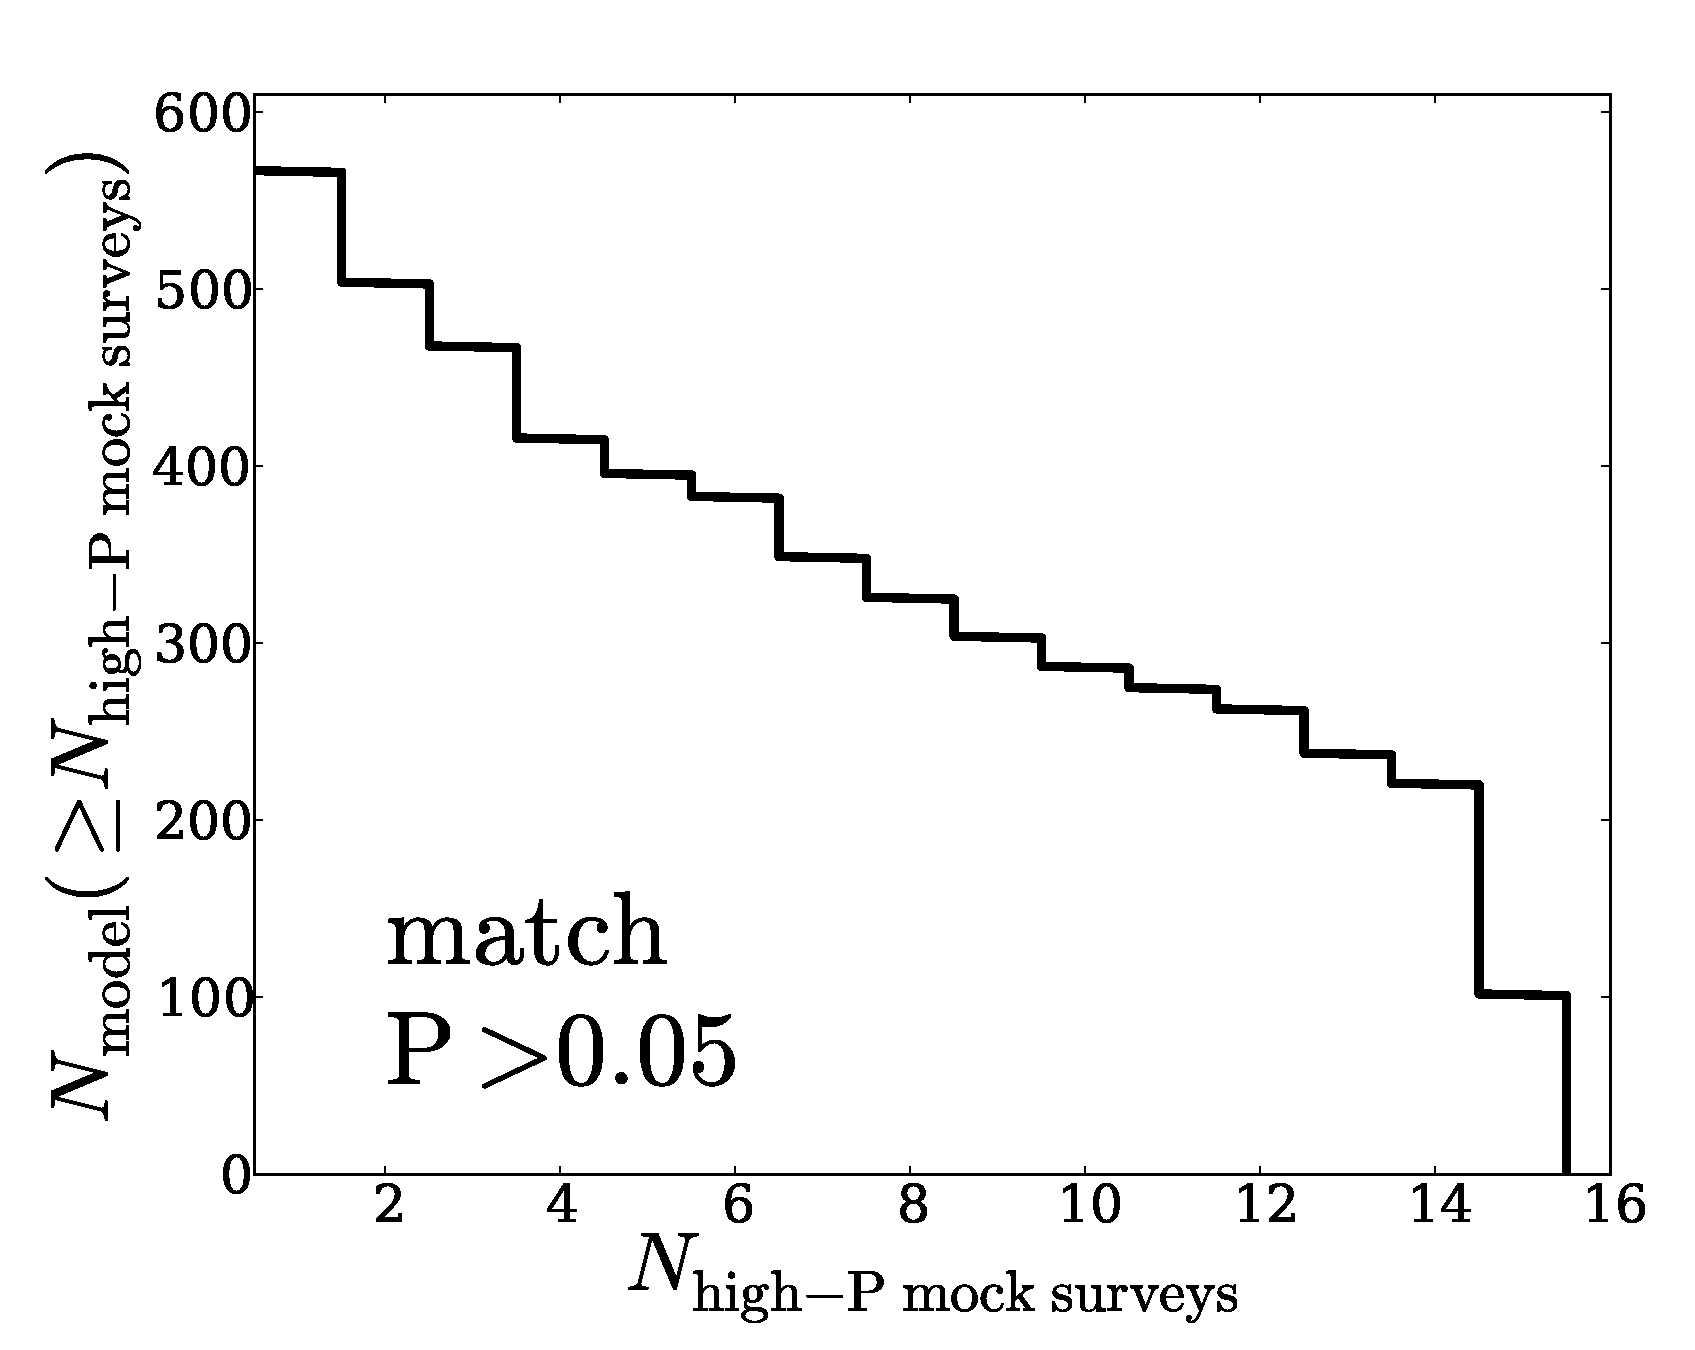
\includegraphics[width=0.95\linewidth,angle=0]{Fig4_match_P5.pdf}
\end{center} 
\caption{ Number of models with at least $N_{\rm high-P}$ mock surveys
  consistent with the observed surface number density
  distribution in terms of the KS-test values $P>0.05$. Only $\sim
  100$ models have all their mocks consistent with observations. 
  \label{fig:high_success_rate}.}  
\end{figure}
 
\subsection{Models with the largest number of consistent mock surveys}

In the previous sub-section we presented a conservative criterion of
agreement by selecting the models that had at least one mock survey
with $P>0.05$ in the KS test. Now we turn to a more strict selection
by requiring all constructed mock surveys to be consistent with
observations. 


Figure \ref{fig:high_success_rate} shows the number of models
that have at least $N_{\rm high-P}$ mocks with $P>0.05$. For each
model ${\mathcal M}$ there are 15 different mock surveys.  We discard
the models that have 14 mocks or less consistent with
observations. With this cut we find $\sim 100$ models with all the 15
mock survey realizations with $P>0.05$.  This cut represents a
reduction by a factor of $\sim 6$ with respect to the total number of
models with at least one consistent mock.   

Figure \ref{fig:restriction_mock} presents the locii of these models
in the parameter space $M_{\rm min}-M_{\rm max}$ and $M_{\rm
  min}-f_{\rm occ}$. With this constraints the
number of consistent models with  $10.5 < \log_{10}M_{\rm min}< 11.0$ are
greatly reduced. This corresponds to the regions in the parameter
space in Figure \ref{fig:landscape} that already had a low number of
consistent mock surveys. On the other hand, from the right panel in
Figure \ref{fig:restriction_mock} one can see that the reduction of
favored values for the occupation fraction $f_{\rm occ}$ is not strong. 

We conclude that conditions on the number density statistics, even if they are
very strict, only put strong constraints on the minimum mass $M_{\rm
  min}$ but not on the other two parameter of the model $M_{\rm max}$
and $f_{\rm occ}$. In the next section we use additional observational
information to constrain these parameters.

\begin{figure*}
\begin{center}
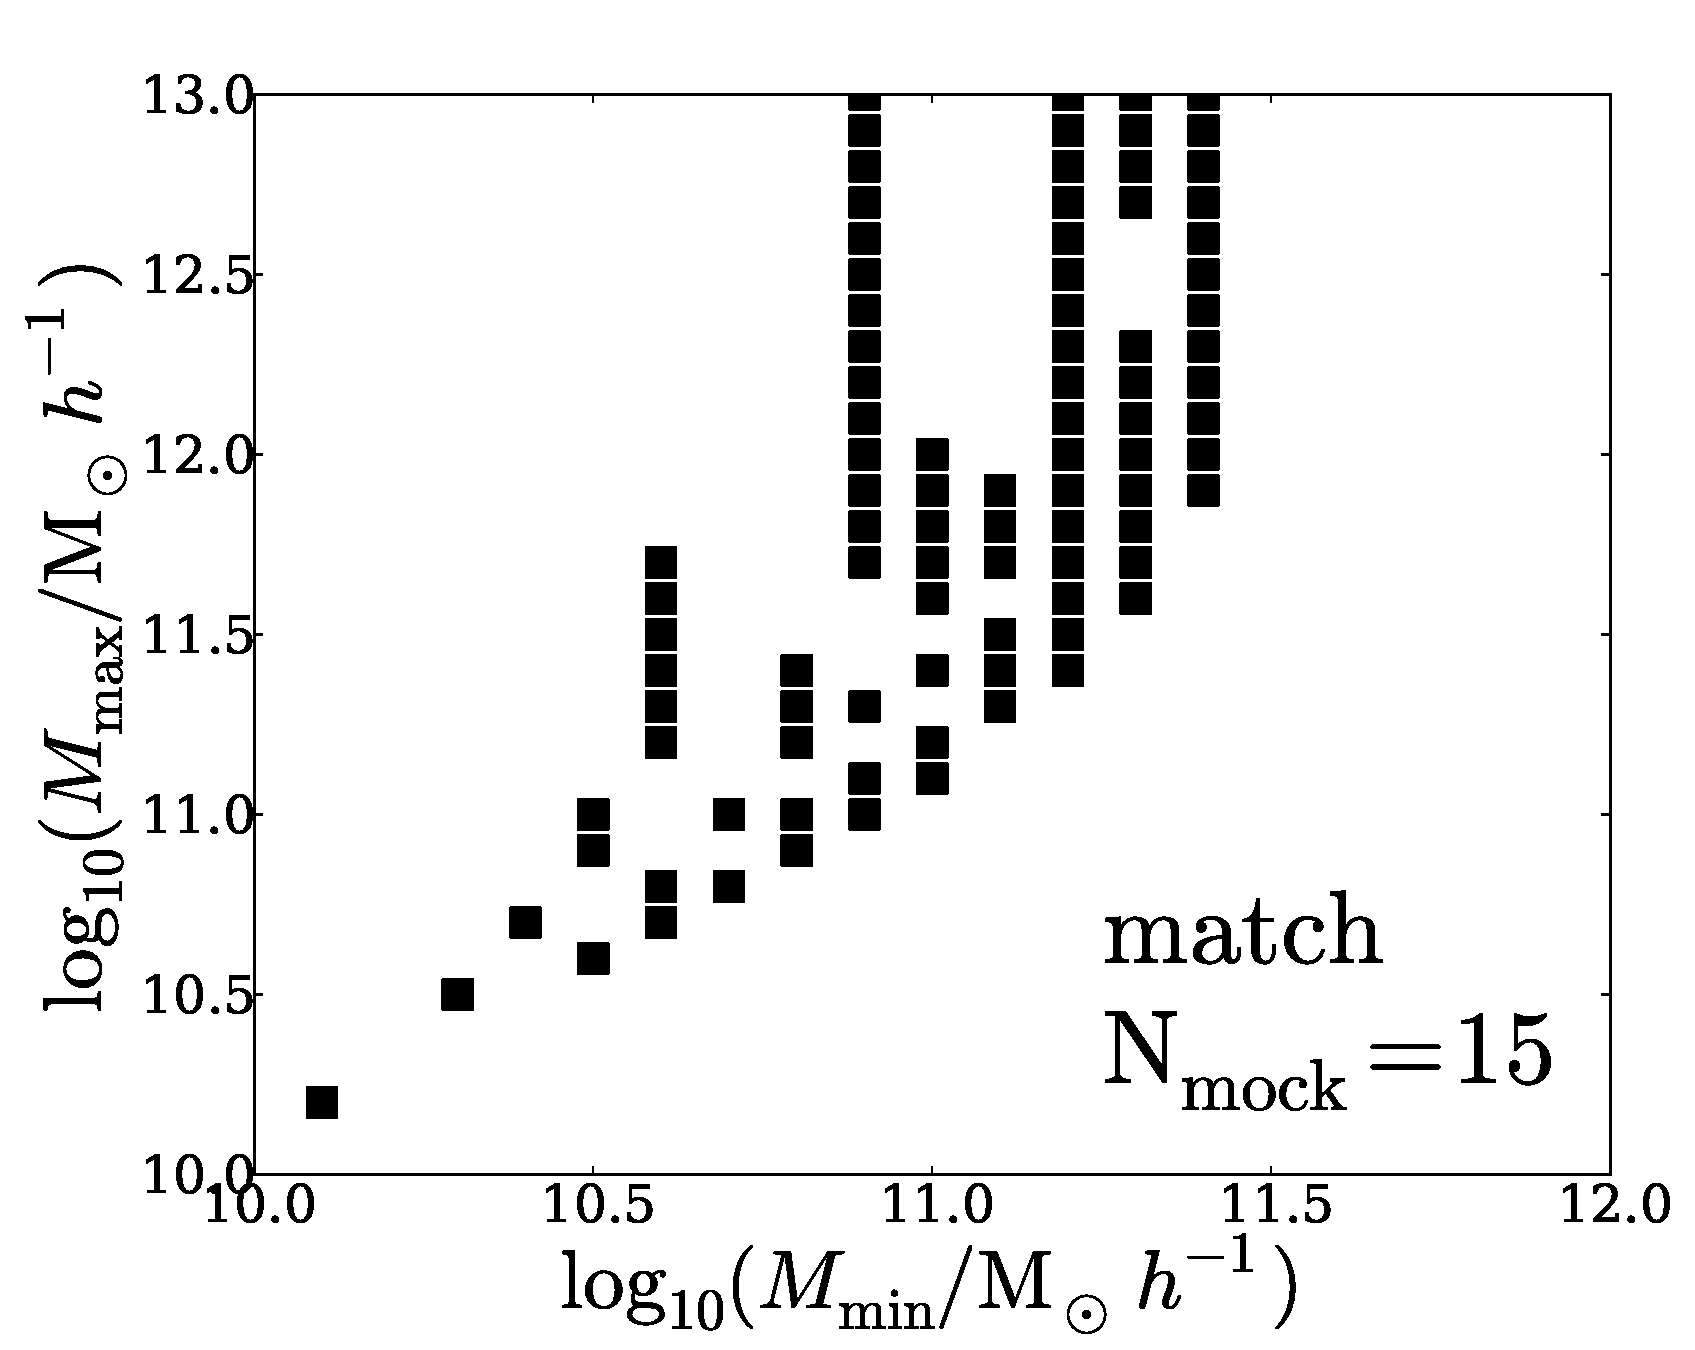
\includegraphics[width=0.46\linewidth,angle=0]{Fig5_match_mass_mock.pdf} 
\hspace{5mm}
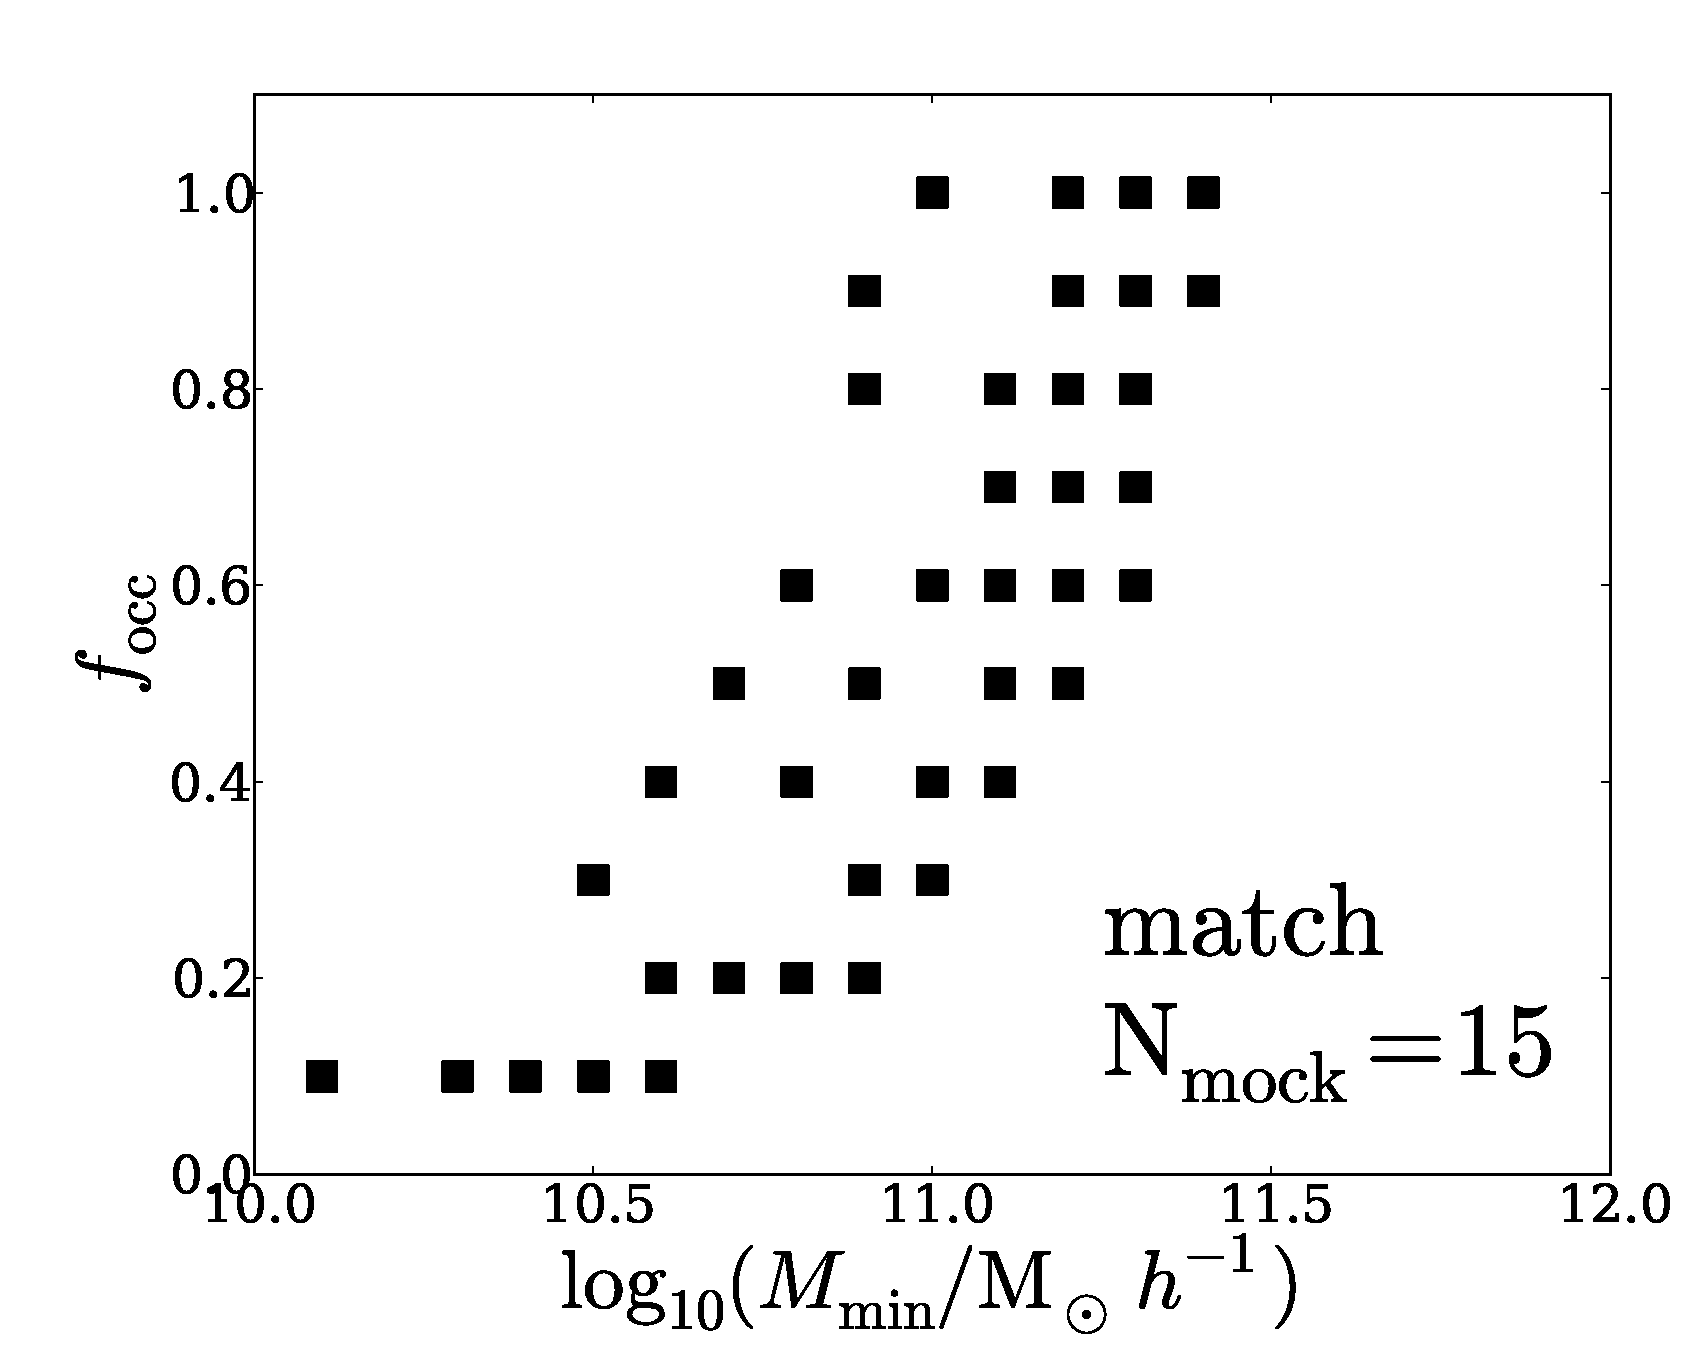
\includegraphics[width=0.46\linewidth,angle=0]{Fig5_match_f_occ_mock.pdf}
\end{center}  
\caption{Favored regions in parameter space when the constraints on
  the maximal number of consistent mocks is imposed. Only the results
  for the {\texttt{match}} method are shown.
  \label{fig:restriction_mock}}  
\end{figure*}



\subsection{Consistency with the Angular Correlation Function}



\begin{figure*}
\begin{center}
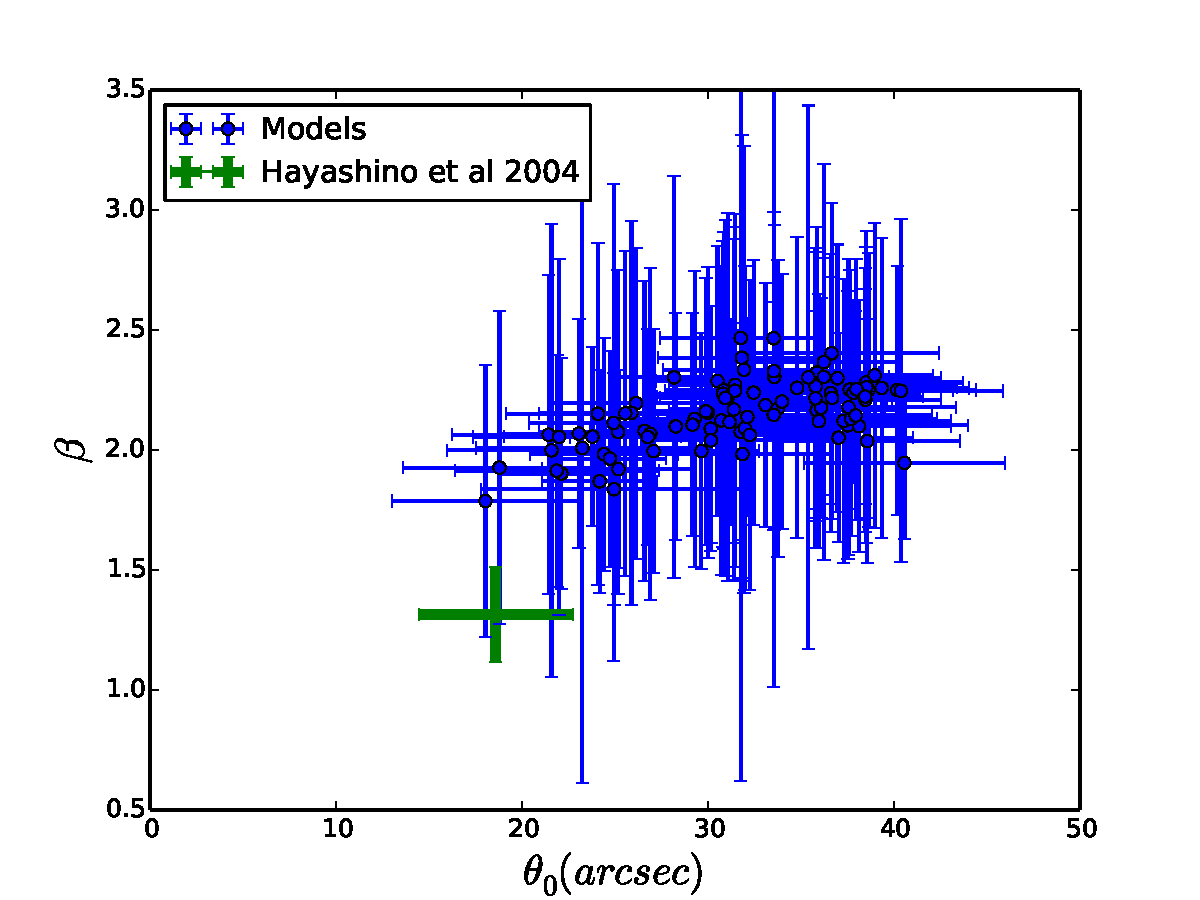
\includegraphics[width=0.46\linewidth,angle=0]{power_law_correlation_maxden.pdf} 
\hspace{5mm}  
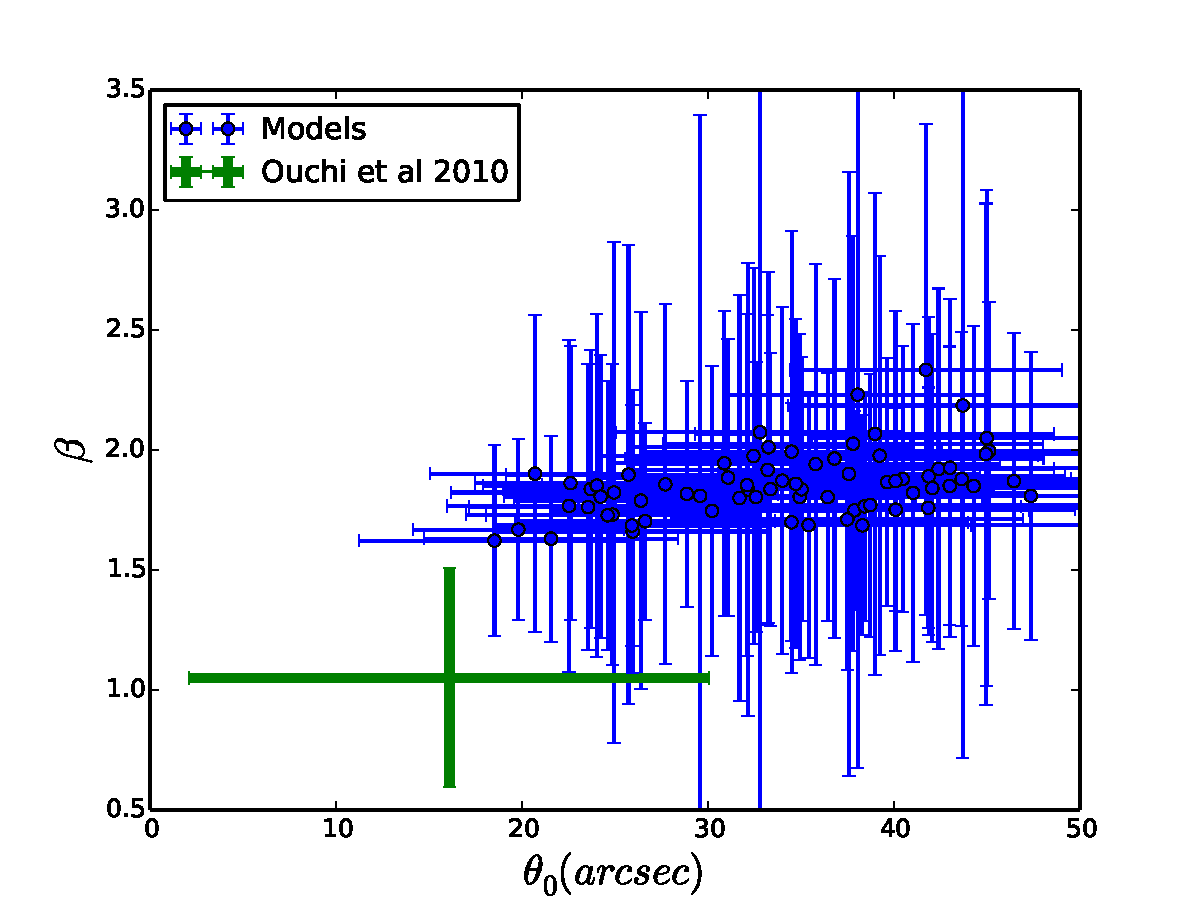
\includegraphics[width=0.46\linewidth,angle=0]{power_law_correlation_meanden.pdf} 
\end{center}
\caption{Values for the free parameters $\theta_{0}$ and $\beta$
in the fitting formula (Eq. \ref{eq:fitting}) for the angular
correlation function. Blue dots correspond to simulations and the
green cross to observations by \citet{Hayashino2004} (left) and
\citet{Ouchi2010} (right). The error bars in the theoretical data correspond
to the quadratic average of the fitting errors for each mock survey
\label{fig:correlation_parameters}}
\end{figure*} 


\begin{figure*}
\begin{center}
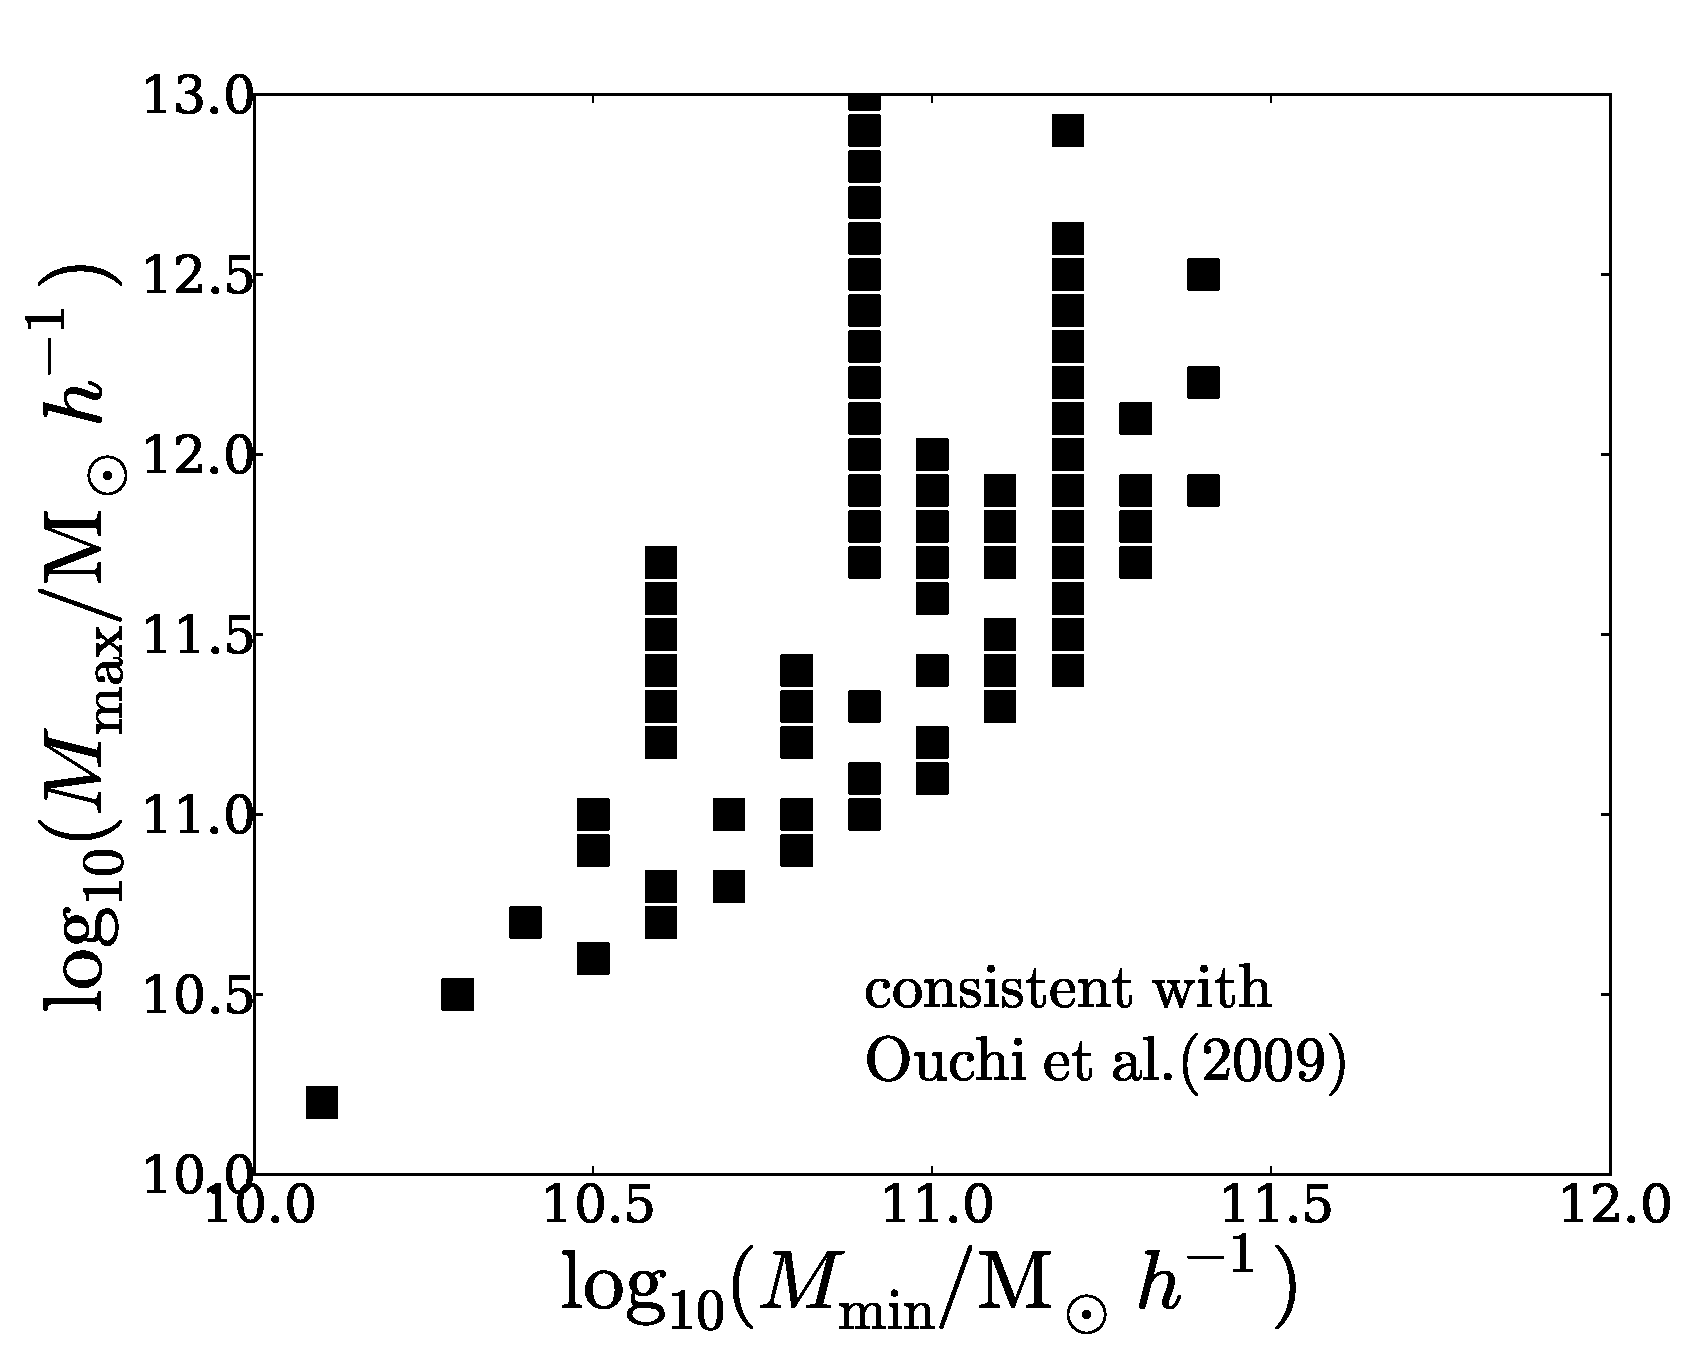
\includegraphics[width=0.46\linewidth,angle=0]{Fig6_meanden_mass.pdf}
\hspace{5mm}
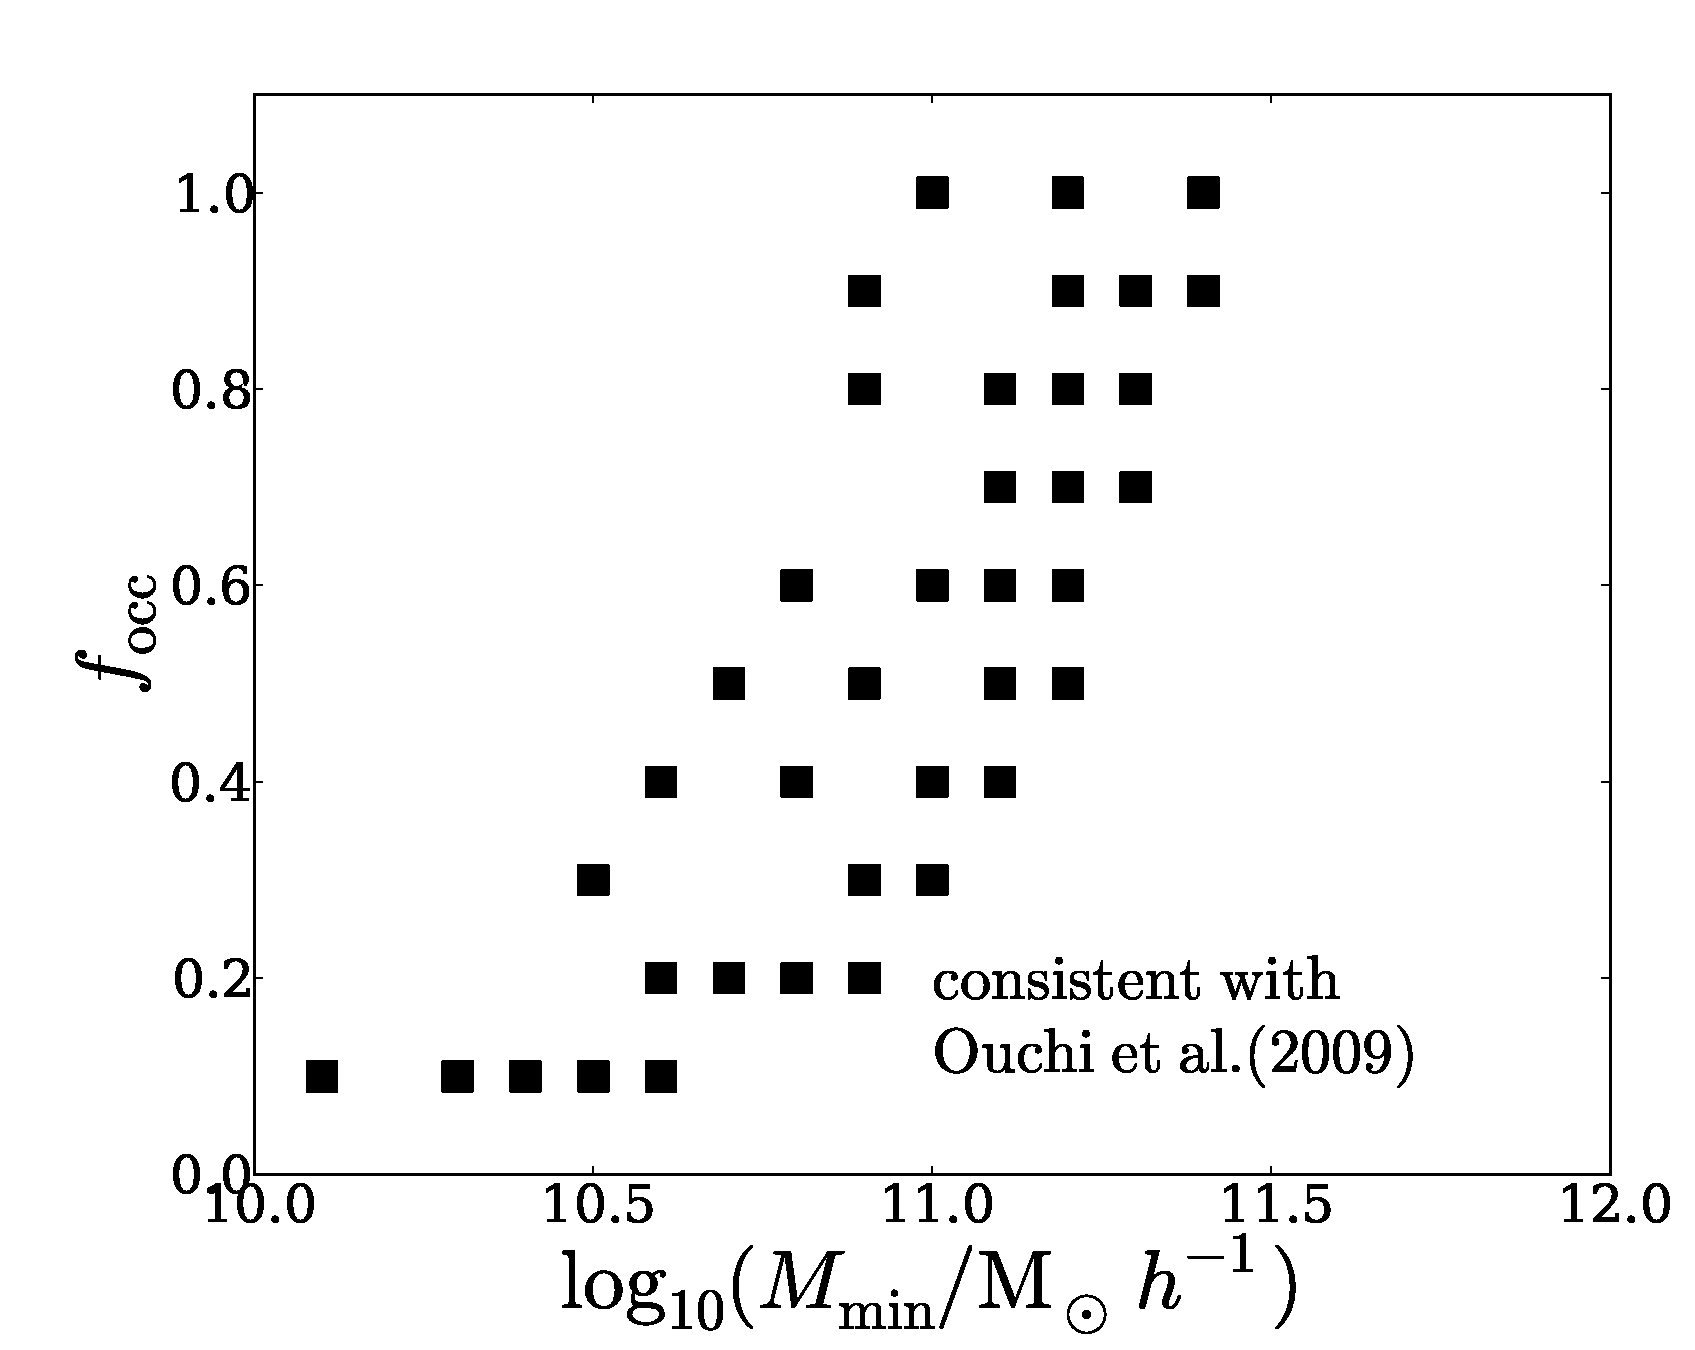
\includegraphics[width=0.46\linewidth,angle=0]{Fig6_meanden_f_occ.pdf}
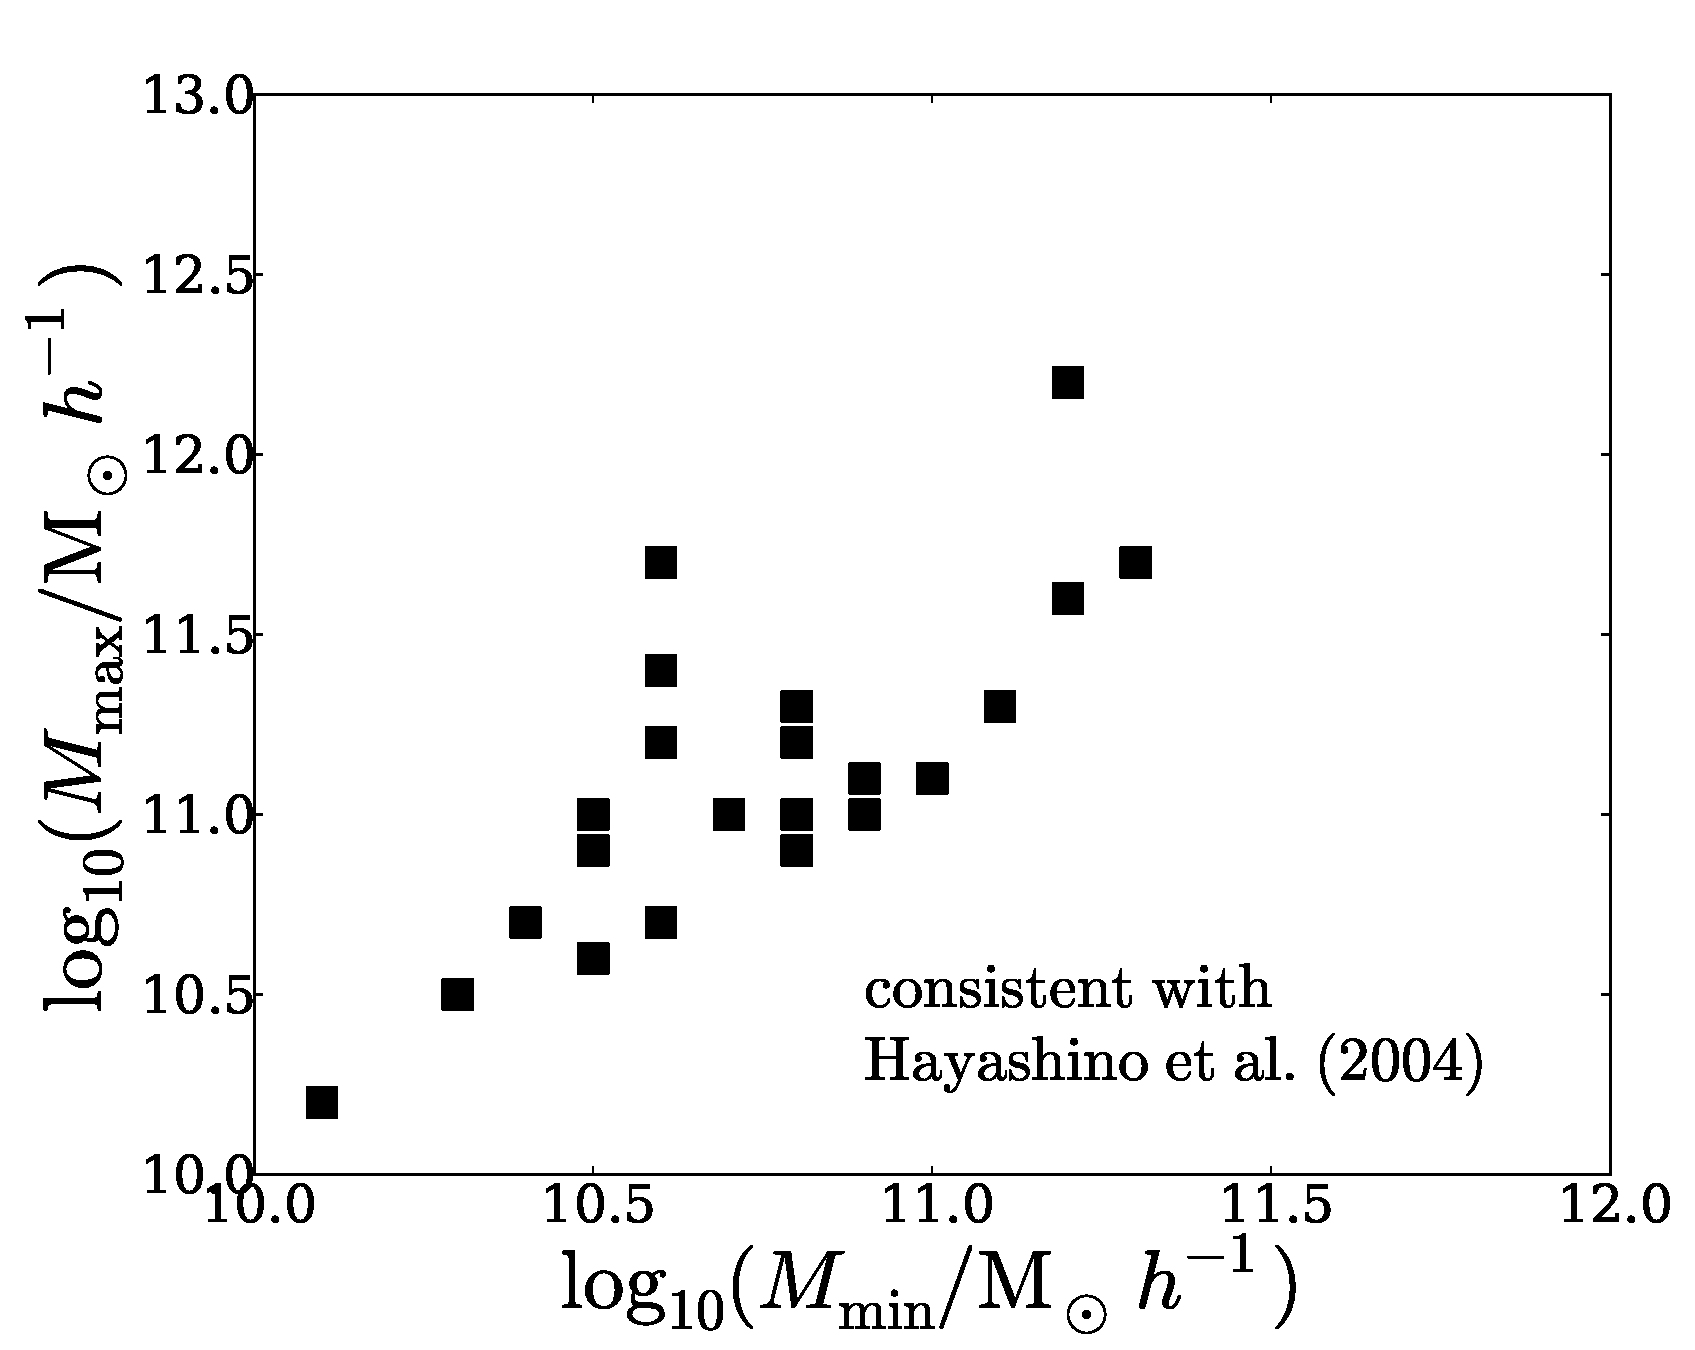
\includegraphics[width=0.46\linewidth,angle=0]{Fig6_maxden_mass.pdf}
\hspace{5mm}
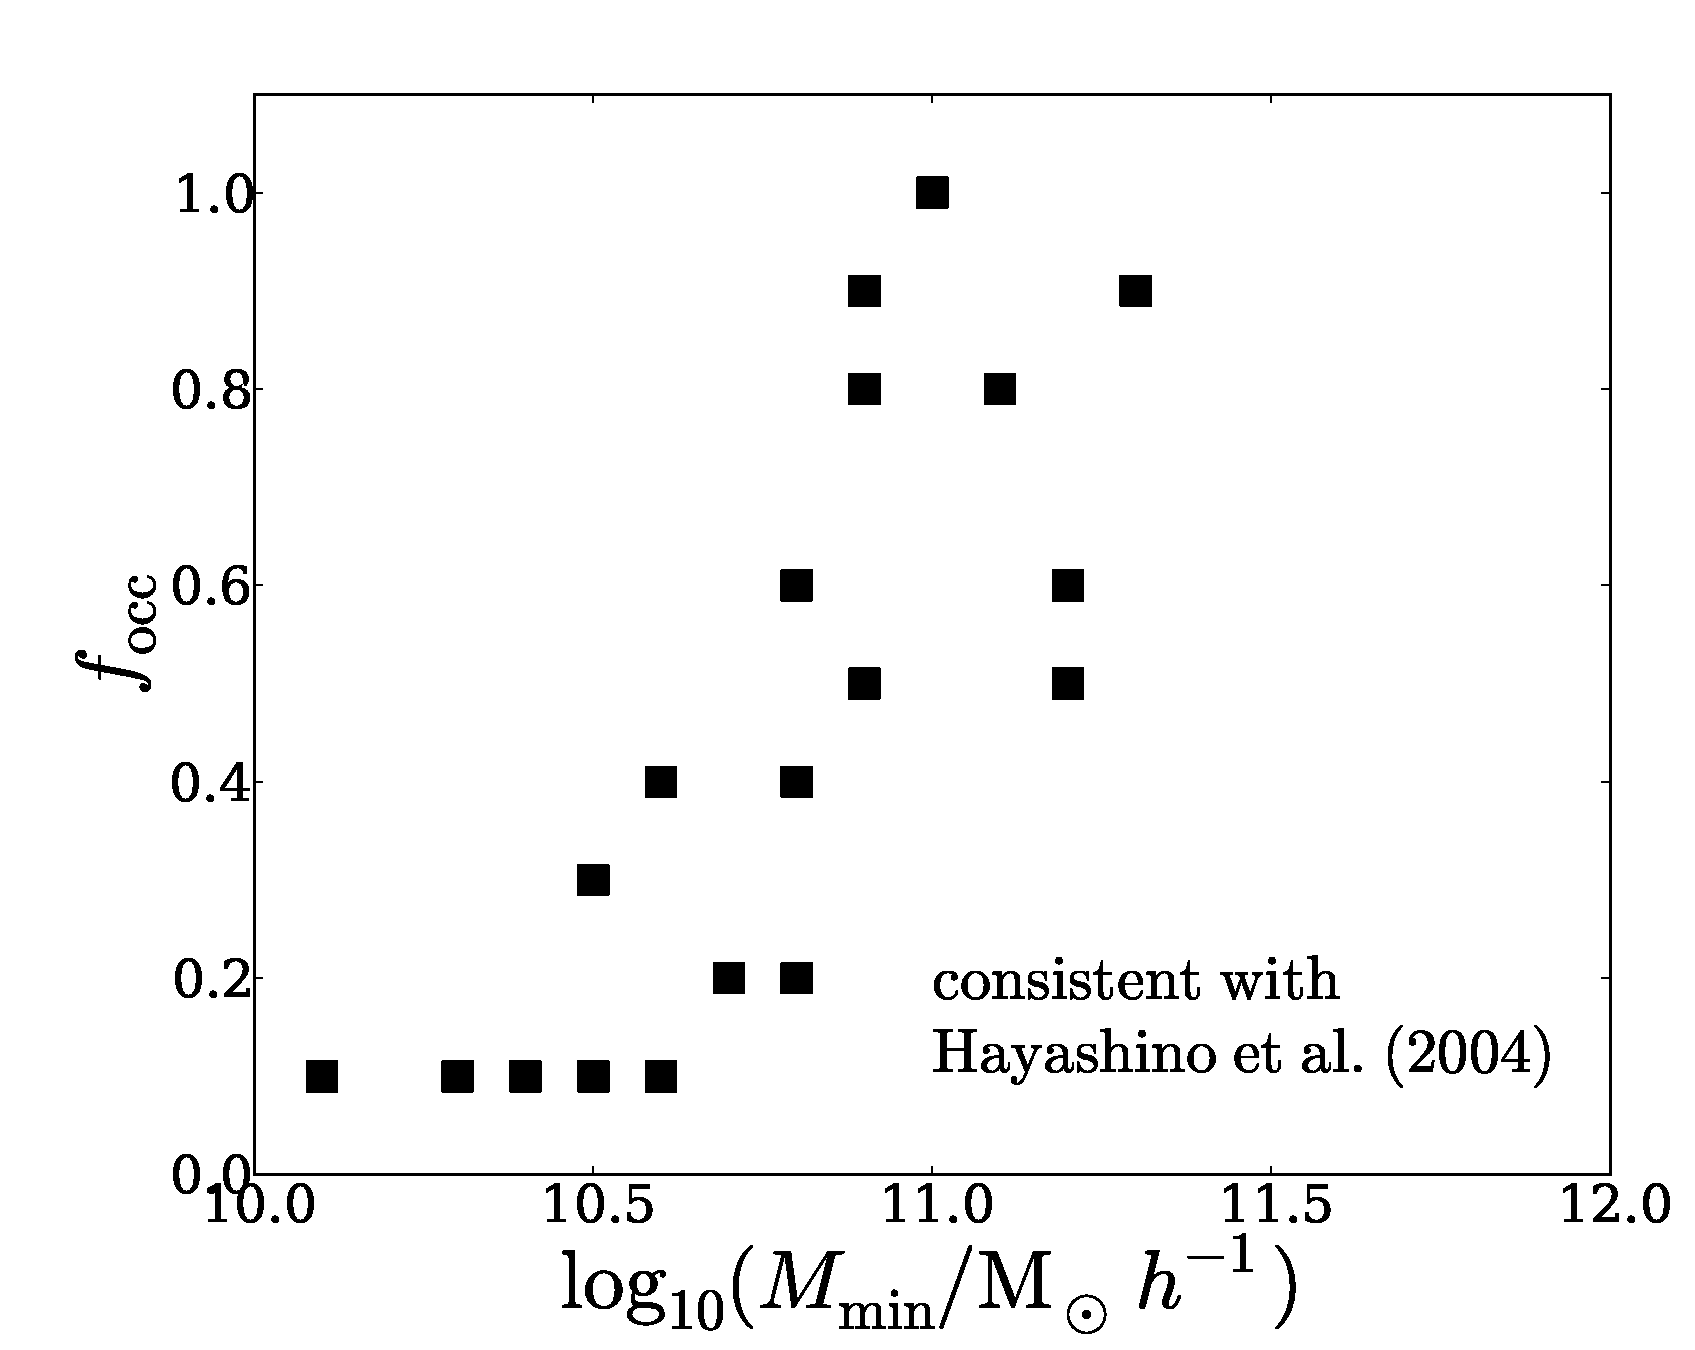
\includegraphics[width=0.46\linewidth,angle=0]{Fig6_maxden_f_occ.pdf}
\end{center}
\caption{Planes $M_{\rm min}$-$M_{\rm max}$ (left) and $M_{\rm
    min}$-$f_{\rm occ}$ (right). with the models fulfilling both
   constraints on the maximal number of consistent mocks and the
  angular correlation function. Upper panels correspond
  checks the consistency with the observational data of
  \citet{Ouchi2010}. Lower panels show results after comparison
  against \citet{Hayashino2004}
  \label{fig:restriction_mock_and_f_occ_corr}} 
\end{figure*} 


Figure \ref{fig:correlation_parameters} shows the main results in a
$\theta_{0}-\beta$  plane where the average and standard deviation
over the mocks is shown in comparison with the result derived from
observations. In the left panel Figure \ref{fig:correlation_parameters} we see
how the observational ACF measured by \cite{Hayashino2004} 
can be successful in reducing the total number of possible models. The
right panel shows the results for fields in the mock catalog with an
average number density compared against the fit of the data
reported by \cite{Ouchi2010}. In this case we find that there are
large uncertainties coming from the observational data, and only a reduced
fraction of the models can be discarded.


In Figure \ref{fig:restriction_mock_and_f_occ_corr} we present the preferred
models in the planes $M_{\rm min}$-$M_{\rm  max}$ and $M_{\rm min}$-$f_{\rm occ}$
both for the comparisons against \cite{Hayashino2004} and
\cite{Ouchi2010}. To make this selection we consider that
a model is consistent with observations if there is a $1$-$\sigma$
overlap between both the correlation length $\theta_0$ and the power
$\beta$. We clearly see from this Figure that the conditions imposed
by \cite{Hayashino2004} are the tightest. Comparing this Figure with
the results shown in Figure \ref{fig:restriction_mock} we see that
practically all models with $M_{\rm max}>10^{12}$ are removed. On the
other hand the comparison against \cite{Ouchi2010} does not
substantially reduce the number of models. 

At this point we take the most strict decision to keep 
models consistent with both observational constraints. This
reduces the selection to the models already restricted by
the data in \cite{Hayashino2004} as presented in the lower panels of Figure
\ref{fig:restriction_mock_and_f_occ_corr}. Our main conclusions after
this comparison is that clustering information is able to put
meaningful constraints on the values of $M_{\rm max}$. However, the
possible values for the occupation fraction, despite having a strong correlation
with $M_{\rm min}$, still are in the initial range $0.1\leq f_{\rm
  occ}\leq 1$. 

\section{Discussion}

In the previous Section we started by matching the rough numbers for the
galaxy surface number density. This sets the median mass of all
successful models to the broad range $(10^{10}$-$10^{12})$ \hMsun for
$M_{\rm min}$ and $M_{\rm max}$. Then we included additional criteria on the
number of mock surveys that must be consistent observations
and the information from the angular correlation function, reducing
the number of feasible models. We ended up with $23$ models out of
the initial $9000$ possible combination of parameters. 

Now we define the halo mass range $\Delta M=\log_{10}M_{\rm max} -
\log_{10}M_{\rm  min}$, to use it together with the occupation
fraction, $f_{\rm occ}$, and the minimum mass $M_{\rm min}$ to
classify all the successful models into two families:   


\begin{itemize}
\item[(1)] Low $f_{\rm occ}\leq 0.3$, $M_{\rm min}\leq 10^{10.8}\hMsun$ and low $\Delta M\leq 1.0$
  dex: 12 models. 
\item[(2)] High $f_{\rm occ}> 0.3$, $M_{\rm min}\geq 10^{10.8}\hMsun$ and
  low $\Delta M\leq 1.0$: 11 models 
\end{itemize}
%
The full list of parameter in the two families is summarized in Table
\ref{table:firstfamily} and Table \ref{table:secondfamily}. We do not
have a clear majority of any family. This leads us to the following
two conclusions. First, the occupation fraction cannot be constrained
based on clustering analysis. Second, the halos hosting LAEs have a
narrow mass range.  

The existence of a narrow mass range for halo masses has different
possible explanations. A cut at the low mass end, $M_{\rm min}$, can be
interpreted in terms of the minimal halo star formation rate needed to
produce the \ly luminosity needed to be above a given detection
threshold.  However, under the reasonable assumption of star formation
rate increasing with halo mass, the cut at higher halo masses $M_{\rm
  max}$requires a different justification. There are two complementary physical
scenarios that could provide it.

One scenario can be presented in terms of a decreasing escape fraction
of \ly radiation in massive systems. Detailed galaxy formation models
support the idea that massive galaxies with higher metallicities have
larger dust contents and less concentrated ISM than lower mass
systems. Due to the resonant nature of the \ly line the probability of
absorption  of \ly photons increases in massive systems, producing
high absorption of the \ly line but not of UV continuum or other
non-resonant lines \citep{Laursen2009,ForeroRomero2011}. In a second
scenario larger systems have more extended gaseous envelopes which due
to resonance effects of the \ly line, induces a low surface brightness
and a broader line, making these systems less observable in narrow
band filter surveys \citep{Laursen2009,Zheng2010}.    


\subsection{Comparison against results from galaxy surveys}

Theoretical interpretations of blind galaxy surveys at $z=2.2$ find a
volume weighted escape fraction $f_{\rm esc}\sim 0.1-0.2$
\cite{Hayes2010}, similar results are obtained in a recent theoretical
study of observational data in a wide redshift range $0<z<6$
\citep{Dijkstra2013}. 


\cite{Hayes2010} showed that the luminosity function for
LAEs at $z=2.2$ is consistent with the escape fraction being constant
for every galaxy regardless of its luminosity. From this results they
derive that almost $90\%$ of the star forming galaxies emit insufficient
Lyman $\alpha$ to be detected, effectively setting the occupation
fraction to be $f_{\rm occ}=0.10$. \cite{Dijkstra2013} use similar
methods to find an average \ly escape fraction in high-z galaxies,
they conclude that there is a range in \ly luminosity where the escape
fraction they derive at $z\sim 3.0$, $f_{\rm esc}=(17\pm 5)\%$, could
be interpreted as an occupation fraction $f_{\rm occ}\sim 0.2$. We
consider a success that our model indeed includes such low occupation
fraction models. The observational evidence from galaxy surveys seem
to disfavor the second family of models with high occupation
fractions. Nevertheless, it remains an open task to explain the narrow
mass range $\Delta M<0.5$ in most of the models. 


\subsection{Comparison to other clustering estimates}

Observational evidence based on the ACF inferred from photometric
measurements in the Extended Chandra Deep Field South has shown that
the median dark matter masses of h los hosting LAEs is
$\log_{10}M_{\rm  med}=10.9^{+0.5}_{-0.9}$\Msun, with a corresponding
occupation fraction of $1-10\%$  \citep{Gawiser07}.  \cite{Ouchi2010}
presents analysis of LAE observations in the redshift interval
$3.1<z<7.0$ and at $z=3.1$ They quote an average mass for the host
dark matter halos of $M_{h}=2.9^{+24.0}_{-2.9}\times 10^{10}$ \hMsun
with a corresponding duty cycle of $0.008\pm 0.03$.  

Our results are in a general good agreement with those estimates for
the host mass. This is not completely unexpected given that we have
also required consistency with ACF measurements. These expectations
are matched by the first family of models, also summarized in Table
\ref{table:firstfamily}. These models, which favor only the very
low occupations fractions, are also consistent in that regards with
the observational expectations.

The novelty in our results is that we have a detailed estimate for 
host halo mass range together with the escape fraction. This allows us
to demonstrate that the halo mass range can in some cases be narrow $\Delta M <
0.3$dex, something that cannot be inferred from ACF analysis alone.
Furthermore, In contrast to \citep{Gawiser07} and \citep{Ouchi2010} we
find that an ACF analysis on a single data-set is not enough to rule
out models with a high occupation fraction $f_{\rm occ}>0.3$, which
represent half of our best models. 

\begin{table}
\begin{center}
\begin{tabular}{cccc}\hline\hline
$\log_{10}M_{\rm min}$ & $\log_{10}M_{\rm max}$ & $f_{\rm occ}$ & $\Delta M$\\\hline
10.1 &10.2 & 0.1 & 0.1\\
10.3 &10.5 & 0.1 & 0.2\\
10.4 &10.7 & 0.1 & 0.3\\
10.5 &10.6 & 0.3 & 0.1\\
10.5 &10.9 & 0.1 & 0.4\\
10.5 &11.0 & 0.1 & 0.5\\
10.6 &11.2 & 0.1 & 0.6\\
10.6 &11.4 & 0.1 & 0.8\\
10.6 &11.7 & 0.1 & 1.1\\
10.7 &11.0 & 0.2 & 0.3\\
10.8 &11.2 & 0.2 & 0.4\\
10.8 &11.3 & 0.2 & 0.5\\\hline
\end{tabular}
\end{center}
\caption{\label{table:firstfamily}List of parameters for the first
  family of models. Narrow mass range $\Delta M\leq 1.0$ dex and low
  occupation fraction $f_{\rm occ}\leq 0.3$.} 
\end{table}



\begin{table}
\begin{center}
\begin{tabular}{cccc}\hline\hline
$\log_{10}M_{\rm min}$ & $\log_{10}M_{\rm max}$ & $f_{\rm occ}$ & $\Delta M$\\\hline
10.6 &10.7 &0.4 & 0.1\\
10.8 &10.9 &0.6 & 0.1\\
10.8 &11.0 &0.4 & 0.2\\
10.9 &11.0 &0.8 & 0.1\\
10.9 &11.0 &0.9 & 0.1\\
10.9 &11.1 &0.5 & 0.2\\
11.0 &11.1 &1.0 & 0.1\\
11.1 &11.3 &0.8 & 0.2\\
11.2 &11.6 &0.6 & 0.4\\
11.2 &12.2 &0.5 & 1.0\\
11.3 &11.7 &0.9 & 0.4\\\hline
\end{tabular}
\end{center}
\caption{\label{table:secondfamily}List of parameters for the second
  family of models. Narrow mass range $\Delta M\leq 1.0$ dex and high occupation fraction $f_{\rm occ}>0.3$.}
\end{table}

\subsection{In the context of abundance matching models}

The abundance matching methods are based on observational results for
Lyman Break Galaxies (LBGs) \citep{Behroozi2013a,Behroozi2013b}.  In
the case of \cite{Behroozi2013a} the minimum halo mass considered to
be relevant in their analysis is $10^{11.4}$\hMsun. They report
stellar mass mass around $(1.0\pm0.3)\times 10^{9.0}$ \hMsun, while
their star formation rate is in the range $0.6\pm 0.2$ \Msun yr$^{-1}$,
which nevertheless are close to the lower bound of values inferred for
LAEs at high redshift \citep{Gawiser2007,Nilsson2009,Pentericci2009}. 

In our results, all the preferred models have a halo mass range lower
than the minimum of $M_{\rm min}<10^{11.4}$\hMsun considered in
abundance matching at $z=3$. Our results confirm the expectations
that most of  LAEs are to be found in less massive halos LBG hosts. A
detailed analysis of the spectral and photometric properties of LAEs
coupled to the kind of analysis performed in this paper can be a guide
in the study of the properties of low mass dark matter halos at
$z=3.1$, extending the capabilities of abundance matching methods.

\subsection{Caveats of our method}

There are two important caveats for the work presented here. The first is the
assumption of a single LAE per dark matter halo. This contradicts the
general expectation of dark matter sub-halos in the simulation to host
satellite galaxies. However, it has been found in analysis based on
the shape of the correlation function \citep{Jose2013b} that satellite
galaxies are not a dominant population, making our initial
approximation a reasonable one. Therefore we conclude that including
the effect of satellite galaxies won't change the main results
reported in this \documentname.

The second caveat are the precise values for the mass intervals. These
values are defined from the halos defined in using the FOF halo
finder. Different halo finders and definitions for the detection
density threshold can yield different masses up to a factor. For
instance a Friends-of-Friends algorithm with linking length $l=0.20$
times the average inter-particle distance finds halos on average $1.4$
times less massive than halos defined  with an spherical overdensity
algorithm halos \citep{Bolshoi}. Therefore, the mass values for
$M_{\rm min}$ and $M_{\rm max}$ should not be considered exact within
less than $\sim 0.2$ dex.  



\subsection{On the reproducibility of our results}

All the software, raw and processed data to produce the results
and plots in this paper are publicly available in a github
repository \footnote{https://github.com/forero/CosmicVarianceLAES}. Most
of the code to produce the plots can be found as an Ipython notebook
\citep{IPython} in the same repository.



\section{Conclusions}
\label{sec:conclusions}

In this \documentname we look for constraints on the preferred mass
and occupation fraction of dark matter halos hosting Lyman Alpha Emitters at
redshift $z=3.1$ in a $\Lambda$CDM cosmology. We perform this study
paying special attention to the impact of cosmic variance on these
results. To this end we build a large number of mock catalogs matching
observational geometries. The mocks are constructed from a N-body simulation
following a simple recipe to assign a single LAE to each halo. Only
a fraction $f_{\rm occ}$ of halos with a mass range  $M_{\rm
  min}<M_{\rm h}<M_{\rm   max}$ can host a LAE. We proceed with a
thorough exploration of the space of free parameters $M_{\rm min},
M_{\rm max}$ and $f_{\rm occ}$ to find mocks that are consistent with
two observational constraints: the surface number density and the
angular correlation function. Out of the initial $9000$ 
combinations of parameters in the model we find $23$ arrangements
consistent with observations.

We find that the observational information we use is insufficient to
impose a tight constraint on the escape fraction. On the other hand
the minimum mass and maximum mass are tightly constrained as follows
$M_{\rm max}<10^{12}$\hMsun and $10^{10}\hMsun\leq M_{\rm min}\leq
10^{11.5}\hMsun$. Furthermore, we find that the mass range defined as
$\Delta M=\log_{10}M_{\rm max} - \log_{10}M_{\rm min}$ is always
$\Delta M\leq 1.0$.

The wide range in solutions is facilitated by the large dispersion in
the statistics derived from the mocks. Nevertheless, all the halo mass
ranges and occupation fractions deduced previous analysis
\citep[i.e.][]{Gawiser2007,Ouchi2010} are a subset of the models we
find in this \documentname. All of our models support the notion that
the most massive halos at $z=3.1$ do not host the brightest LAEs.

The existence of a narrow mass range for halos hosting LAEs, $\Delta
M\leq 1.0$ dex, has two different explanations at least. The
first is having LAEs with a decreasing \ly escape fraction with
increasing mass, the second is having larger screening effects by
neutral Hydrogen around the most massive systems
\citep{Laursen2009,ForeroRomero2011}.   

However, there are extreme cases with a very narrow $\Delta M<0.3$, meaning that
there is barely a factor of $\sim 2$ between the minimum and halo
mass. If these models turn out to be confirmed, this would be a great
challenge for galaxy formation models to explain how is that LAEs can
be hosted in such a narrow range of halo mass. 

In summary, we show how spatial information of LAEs cannot
put a tight constraint on their host halos and occupation fraction. We
foresee that the new observations with new instruments (such as MUSE,
Hyper SuprimeCam and HETDEX) covering larger fields and a wider range
of luminosities will be key in imposing tighter constraints on the
properties of dark matter halos hosting LAEs. At the same time,
additional modeling for \ly radiation transfer , is needed to put a
tighter constrain on the \ly escape fraction in high redshift
galaxies, also paying attention to newly framed physical phenomena, such as the
stochasticity \citep{ForeroRomero2013} in the star formation process,
which might play a role in inducing detection biases in high redshift LAEs.


\section*{Acknowledgments} 
J.E.F-R thanks the hospitality of Changbom Park and the Korea
Institute for Advanced Study where the first full draft of this paper
was completed. The authors also thank Peter Laursen, Paulina Lira, 
Alvaro Orsi and Mark Dijkstra for helpful comments on the physical
interpretation and presentation of our results. J.E.F-R was
supported by the FAPA grant by Vicerrector\'ia de Investigaciones at
Universidad de los Andes.

The MultiDark Database used in this paper and the web application
providing online access to it were constructed as part of the
activities of the German Astrophysical Virtual Observatory as result
of a collaboration between the Leibniz-Institute for Astrophysics
Potsdam (AIP) and the Spanish MultiDark Consolider Project
CSD2009-00064. The Bolshoi and MultiDark simulations were run on the
NASA's Pleiades supercomputer at the NASA Ames Research Center.



\bibliographystyle{mn2e}
\begin{thebibliography}{}

\bibitem[\protect\citeauthoryear{{Behroozi}, {Wechsler} \& {Conroy}}{{Behroozi}
  et~al.}{2013a}]{Behroozi2013b}
{Behroozi} P.~S.,  {Wechsler} R.~H.,    {Conroy} C.,  2013a, \apjl, 762, L31

\bibitem[\protect\citeauthoryear{{Behroozi}, {Wechsler} \& {Conroy}}{{Behroozi}
  et~al.}{2013b}]{Behroozi2013a}
{Behroozi} P.~S.,  {Wechsler} R.~H.,    {Conroy} C.,  2013b, \apj, 770, 57

\bibitem[\protect\citeauthoryear{{Colberg}, {White}, {Yoshida}, {MacFarland},
  {Jenkins}, {Frenk}, {Pearce}, {Evrard}, {Couchman}, {Efstathiou}, {Peacock},
  {Thomas} \& {Virgo Consortium}}{{Colberg} et~al.}{2000}]{Colberg00}
{Colberg} J.~M.,  {White} S.~D.~M.,  {Yoshida} N.,  {MacFarland} T.~J.,
  {Jenkins} A.,  {Frenk} C.~S.,  {Pearce} F.~R.,  {Evrard} A.~E.,  {Couchman}
  H.~M.~P.,  {Efstathiou} G.,  {Peacock} J.~A.,  {Thomas} P.~A.,    {Virgo
  Consortium} 2000, \mnras, 319, 209

\bibitem[\protect\citeauthoryear{{Dayal}, {Ferrara}, {Saro}, {Salvaterra},
  {Borgani} \& {Tornatore}}{{Dayal} et~al.}{2009}]{Dayal2009}
{Dayal} P.,  {Ferrara} A.,  {Saro} A.,  {Salvaterra} R.,  {Borgani} S.,
  {Tornatore} L.,  2009, \mnras, 400, 2000

\bibitem[\protect\citeauthoryear{{Dijkstra} \& {Jeeson-Daniel}}{{Dijkstra} \&
  {Jeeson-Daniel}}{2013}]{Dijkstra2013}
{Dijkstra} M.,  {Jeeson-Daniel} A.,  2013, ArXiv e-prints

\bibitem[\protect\citeauthoryear{{Dijkstra} \& {Kramer}}{{Dijkstra} \&
  {Kramer}}{2012}]{Dijkstra2012}
{Dijkstra} M.,  {Kramer} R.,  2012, \mnras, 424, 1672

\bibitem[\protect\citeauthoryear{{Dijkstra}, {Mesinger} \& {Wyithe}}{{Dijkstra}
  et~al.}{2011}]{Dijkstra11}
{Dijkstra} M.,  {Mesinger} A.,    {Wyithe} J.~S.~B.,  2011, \mnras, 414, 2139

\bibitem[\protect\citeauthoryear{{Forero-Romero} \& {Dijkstra}}{{Forero-Romero}
  \& {Dijkstra}}{2013}]{ForeroRomero2013}
{Forero-Romero} J.~E.,  {Dijkstra} M.,  2013, \mnras, 428, 2163

\bibitem[\protect\citeauthoryear{{Forero-Romero}, {Yepes}, {Gottl{\"o}ber},
  {Knollmann}, {Cuesta} \& {Prada}}{{Forero-Romero}
  et~al.}{2011}]{ForeroRomero2011}
{Forero-Romero} J.~E.,  {Yepes} G.,  {Gottl{\"o}ber} S.,  {Knollmann} S.~R.,
  {Cuesta} A.~J.,    {Prada} F.,  2011, \mnras, 415, 3666

\bibitem[\protect\citeauthoryear{{Forero-Romero}, {Yepes}, {Gottl{\"o}ber} \&
  {Prada}}{{Forero-Romero} et~al.}{2012}]{ForeroRomero2012}
{Forero-Romero} J.~E.,  {Yepes} G.,  {Gottl{\"o}ber} S.,    {Prada} F.,  2012,
  \mnras, 419, 952

\bibitem[\protect\citeauthoryear{{Garel}, {Blaizot}, {Guiderdoni}, {Schaerer},
  {Verhamme} \& {Hayes}}{{Garel} et~al.}{2012}]{Garel2012}
{Garel} T.,  {Blaizot} J.,  {Guiderdoni} B.,  {Schaerer} D.,  {Verhamme} A.,
  {Hayes} M.,  2012, \mnras, 422, 310

\bibitem[\protect\citeauthoryear{{Gawiser}, {Francke}, {Lai}, {Schawinski},
  {Gronwall}, {Ciardullo}, {Quadri}, {Orsi}, {Barrientos}, {Blanc}, {Fazio} \&
  {Feldmeier}}{{Gawiser} et~al.}{2007}]{Gawiser2007}
{Gawiser} E.,  {Francke} H.,  {Lai} K.,  {Schawinski} K.,  {Gronwall} C.,
  {Ciardullo} R.,  {Quadri} R.,  {Orsi} A.,  {Barrientos} L.~F.,  {Blanc}
  G.~A.,  {Fazio} G.,    {Feldmeier} J.~J.,  2007, \apj, 671, 278

\bibitem[\protect\citeauthoryear{{Gawiser}, {Francke}, {Lai}, {Schawinski},
  {Gronwall}, {Ciardullo}, {Quadri}, {Orsi}, {Barrientos}, {Blanc}, {Fazio},
  {Feldmeier}, {Huang}, {Infante}, {Lira} \& {Padilla}}{{Gawiser}
  et~al.}{2007}]{Gawiser07}
{Gawiser} E.,  {Francke} H.,  {Lai} K.,  {Schawinski} K.,  {Gronwall} C.,
  {Ciardullo} R.,  {Quadri} R.,  {Orsi} A.,  {Barrientos} L.~F.,  {Blanc}
  G.~A.,  {Fazio} G.,  {Feldmeier} J.~J.,  {Huang} J.-s.,  {Infante} L.,
  {Lira} P.,    {Padilla} N.,  2007, \apj, 671, 278

\bibitem[\protect\citeauthoryear{{Guaita}, {Francke}, {Gawiser}, {Bauer},
  {Hayes}, {{\"O}stlin} \& {Padilla}}{{Guaita} et~al.}{2013}]{Guaita2013}
{Guaita} L.,  {Francke} H.,  {Gawiser} E.,  {Bauer} F.~E.,  {Hayes} M.,
  {{\"O}stlin} G.,    {Padilla} N.,  2013, \aap, 551, A93

\bibitem[\protect\citeauthoryear{{Hayashino}, {Matsuda}, {Tamura}, {Yamauchi},
  {Yamada}, {Ajiki}, {Fujita}, {Murayama}, {Nagao}, {Ohta}, {Okamura}, {Ouchi},
  {Shimasaku}, {Shioya} \& {Taniguchi}}{{Hayashino}
  et~al.}{2004}]{Hayashino2004}
{Hayashino} T.,  {Matsuda} Y.,  {Tamura} H.,  {Yamauchi} R.,  {Yamada} T.,
  {Ajiki} M.,  {Fujita} S.~S.,  {Murayama} T.,  {Nagao} T.,  {Ohta} K.,
  {Okamura} S.,  {Ouchi} M.,  {Shimasaku} K.,  {Shioya} Y.,    {Taniguchi} Y.,
  2004, \aj, 128, 2073

\bibitem[\protect\citeauthoryear{{Hayes}, {{\"O}stlin}, {Schaerer},
  {Mas-Hesse}, {Leitherer}, {Atek}, {Kunth}, {Verhamme}, {de Barros} \&
  {Melinder}}{{Hayes} et~al.}{2010}]{Hayes2010}
{Hayes} M.,  {{\"O}stlin} G.,  {Schaerer} D.,  {Mas-Hesse} J.~M.,  {Leitherer}
  C.,  {Atek} H.,  {Kunth} D.,  {Verhamme} A.,  {de Barros} S.,    {Melinder}
  J.,  2010, \nat, 464, 562

\bibitem[\protect\citeauthoryear{{Jarosik}, {Bennett}, {Dunkley}, {Gold},
  {Greason}, {Halpern}, {Hill}, {Hinshaw}, {Kogut}, {Komatsu}, {Larson} \&
  {Limon}}{{Jarosik} et~al.}{2011}]{Jarosik2011}
{Jarosik} N.,  {Bennett} C.~L.,  {Dunkley} J.,  {Gold} B.,  {Greason} M.~R.,
  {Halpern} M.,  {Hill} R.~S.,  {Hinshaw} G.,  {Kogut} A.,  {Komatsu} E.,
  {Larson} D.,    {Limon} M.,  2011, \apjs, 192, 14

\bibitem[\protect\citeauthoryear{{Jose}, {Srianand} \& {Subramanian}}{{Jose}
  et~al.}{2013}]{Jose2013b}
{Jose} C.,  {Srianand} R.,    {Subramanian} K.,  2013, ArXiv e-prints

\bibitem[\protect\citeauthoryear{{Klypin}, {Trujillo-Gomez} \&
  {Primack}}{{Klypin} et~al.}{2011}]{Bolshoi}
{Klypin} A.~A.,  {Trujillo-Gomez} S.,    {Primack} J.,  2011, \apj, 740, 102

\bibitem[\protect\citeauthoryear{{Koehler}, {Schuecker} \&
  {Gebhardt}}{{Koehler} et~al.}{2007}]{Koehler2007}
{Koehler} R.~S.,  {Schuecker} P.,    {Gebhardt} K.,  2007, \aap, 462, 7

\bibitem[\protect\citeauthoryear{{Komatsu}, {Dunkley}, {Nolta}, {Bennett},
  {Gold}, {Hinshaw}, {Jarosik}, {Larson}, {Limon}, {Page}, {Spergel} \&
  {Halpern}}{{Komatsu} et~al.}{2009}]{Komatsu2009}
{Komatsu} E.,  {Dunkley} J.,  {Nolta} M.~R.,  {Bennett} C.~L.,  {Gold} B.,
  {Hinshaw} G.,  {Jarosik} N.,  {Larson} D.,  {Limon} M.,  {Page} L.,
  {Spergel} D.~N.,    {Halpern} M.,  2009, \apjs, 180, 330

\bibitem[\protect\citeauthoryear{{Kudritzki}, {M{\'e}ndez}, {Feldmeier},
  {Ciardullo}, {Jacoby}, {Freeman}, {Arnaboldi}, {Capaccioli}, {Gerhard} \&
  {Ford}}{{Kudritzki} et~al.}{2000}]{Kudritzki2000}
{Kudritzki} R.-P.,  {M{\'e}ndez} R.~H.,  {Feldmeier} J.~J.,  {Ciardullo} R.,
  {Jacoby} G.~H.,  {Freeman} K.~C.,  {Arnaboldi} M.,  {Capaccioli} M.,
  {Gerhard} O.,    {Ford} H.~C.,  2000, \apj, 536, 19

\bibitem[\protect\citeauthoryear{{Landy} \& {Szalay}}{{Landy} \&
  {Szalay}}{1993}]{Landy1993}
{Landy} S.~D.,  {Szalay} A.~S.,  1993, \apj, 412, 64

\bibitem[\protect\citeauthoryear{{Laursen}, {Duval} \& {{\"O}stlin}}{{Laursen}
  et~al.}{2013}]{Laursen2013}
{Laursen} P.,  {Duval} F.,    {{\"O}stlin} G.,  2013, \apj, 766, 124

\bibitem[\protect\citeauthoryear{{Laursen}, {Razoumov} \&
  {Sommer-Larsen}}{{Laursen} et~al.}{2009}]{Laursen2009}
{Laursen} P.,  {Razoumov} A.~O.,    {Sommer-Larsen} J.,  2009, \apj, 696, 853

\bibitem[\protect\citeauthoryear{{Laursen} \& {Sommer-Larsen}}{{Laursen} \&
  {Sommer-Larsen}}{2007}]{Laursen2007}
{Laursen} P.,  {Sommer-Larsen} J.,  2007, \apjl, 657, L69

\bibitem[\protect\citeauthoryear{{Matsuda}, {Yamada}, {Hayashino}, {Tamura},
  {Yamauchi}, {Murayama}, {Nagao}, {Ohta}, {Okamura}, {Ouchi}, {Shimasaku},
  {Shioya} \& {Taniguchi}}{{Matsuda} et~al.}{2005}]{Matsuda2005}
{Matsuda} Y.,  {Yamada} T.,  {Hayashino} T.,  {Tamura} H.,  {Yamauchi} R.,
  {Murayama} T.,  {Nagao} T.,  {Ohta} K.,  {Okamura} S.,  {Ouchi} M.,
  {Shimasaku} K.,  {Shioya} Y.,    {Taniguchi} Y.,  2005, \apjl, 634, L125

\bibitem[\protect\citeauthoryear{{Neufeld}}{{Neufeld}}{1991}]{Neufeld1991}
{Neufeld} D.~A.,  1991, \apjl, 370, L85

\bibitem[\protect\citeauthoryear{{Nilsson}, {M{\o}ller}, {M{\"o}ller}, {Fynbo},
  {Micha{\l}owski}, {Watson}, {Ledoux}, {Rosati}, {Pedersen} \&
  {Grove}}{{Nilsson} et~al.}{2007}]{Nilsson2007}
{Nilsson} K.~K.,  {M{\o}ller} P.,  {M{\"o}ller} O.,  {Fynbo} J.~P.~U.,
  {Micha{\l}owski} M.~J.,  {Watson} D.,  {Ledoux} C.,  {Rosati} P.,  {Pedersen}
  K.,    {Grove} L.~F.,  2007, \aap, 471, 71

\bibitem[\protect\citeauthoryear{{Nilsson}, {Tapken}, {M{\o}ller}, {Freudling},
  {Fynbo}, {Meisenheimer}, {Laursen} \& {{\"O}stlin}}{{Nilsson}
  et~al.}{2009}]{Nilsson2009}
{Nilsson} K.~K.,  {Tapken} C.,  {M{\o}ller} P.,  {Freudling} W.,  {Fynbo}
  J.~P.~U.,  {Meisenheimer} K.,  {Laursen} P.,    {{\"O}stlin} G.,  2009, \aap,
  498, 13

\bibitem[\protect\citeauthoryear{{Orsi}, {Lacey} \& {Baugh}}{{Orsi}
  et~al.}{2012}]{Orsi2012}
{Orsi} A.,  {Lacey} C.~G.,    {Baugh} C.~M.,  2012, \mnras, 425, 87

\bibitem[\protect\citeauthoryear{{Ouchi}, {Shimasaku}, {Akiyama}, {Simpson},
  {Saito}, {Ueda}, {Furusawa}, {Sekiguchi}, {Yamada}, {Kodama}, {Kashikawa},
  {Okamura}, {Iye}, {Takata}, {Yoshida} \& {Yoshida}}{{Ouchi}
  et~al.}{2008}]{Ouchi2008}
{Ouchi} M.,  {Shimasaku} K.,  {Akiyama} M.,  {Simpson} C.,  {Saito} T.,  {Ueda}
  Y.,  {Furusawa} H.,  {Sekiguchi} K.,  {Yamada} T.,  {Kodama} T.,  {Kashikawa}
  N.,  {Okamura} S.,  {Iye} M.,  {Takata} T.,  {Yoshida} M.,    {Yoshida} M.,
  2008, \apjs, 176, 301

\bibitem[\protect\citeauthoryear{{Ouchi}, {Shimasaku}, {Furusawa}, {Saito},
  {Yoshida}, {Akiyama}, {Ono}, {Yamada}, {Ota}, {Kashikawa}, {Iye}, {Kodama},
  {Okamura}, {Simpson} \& {Yoshida}}{{Ouchi} et~al.}{2010}]{Ouchi2010}
{Ouchi} M.,  {Shimasaku} K.,  {Furusawa} H.,  {Saito} T.,  {Yoshida} M.,
  {Akiyama} M.,  {Ono} Y.,  {Yamada} T.,  {Ota} K.,  {Kashikawa} N.,  {Iye} M.,
   {Kodama} T.,  {Okamura} S.,  {Simpson} C.,    {Yoshida} M.,  2010, \apj,
  723, 869

\bibitem[\protect\citeauthoryear{{Peebles}}{{Peebles}}{1980}]{Peebles1980}
{Peebles} P.~J.~E.,  1980, {The large-scale structure of the universe}

\bibitem[\protect\citeauthoryear{{Pentericci}, {Grazian}, {Fontana},
  {Castellano}, {Giallongo}, {Salimbeni} \& {Santini}}{{Pentericci}
  et~al.}{2009}]{Pentericci2009}
{Pentericci} L.,  {Grazian} A.,  {Fontana} A.,  {Castellano} M.,  {Giallongo}
  E.,  {Salimbeni} S.,    {Santini} P.,  2009, \aap, 494, 553

\bibitem[\protect\citeauthoryear{P\'erez \& Granger}{P\'erez \&
  Granger}{2007}]{IPython}
P\'erez F.,  Granger B.~E.,  2007, {C}omput. {S}ci. {E}ng., 9, 21

\bibitem[\protect\citeauthoryear{Riebe, Partl, Enke, Forero-Romero, Gottlöber,
  Klypin, Lemson, Prada, Primack, Steinmetz \& Turchaninov}{Riebe
  et~al.}{2013}]{MultiDark}
Riebe K.,  Partl A.~M.,  Enke H.,  Forero-Romero J.,  Gottlöber S.,  Klypin
  A.,  Lemson G.,  Prada F.,  Primack J.~R.,  Steinmetz M.,    Turchaninov V.,
  2013, Astronomische Nachrichten, 334, 691

\bibitem[\protect\citeauthoryear{{Springel}, {White}, {Jenkins}, {Frenk},
  {Yoshida}, {Gao}, {Navarro}, {Thacker}, {Croton}, {Helly}, {Peacock}, {Cole},
  {Thomas}, {Couchman}, {Evrard}, {Colberg} \& {Pearce}}{{Springel}
  et~al.}{2005}]{SpringelNature05}
{Springel} V.,  {White} S.~D.~M.,  {Jenkins} A.,  {Frenk} C.~S.,  {Yoshida} N.,
   {Gao} L.,  {Navarro} J.,  {Thacker} R.,  {Croton} D.,  {Helly} J.,
  {Peacock} J.~A.,  {Cole} S.,  {Thomas} P.,  {Couchman} H.,  {Evrard} A.,
  {Colberg} J.,    {Pearce} F.,  2005, \nat, 435, 629

\bibitem[\protect\citeauthoryear{{Verhamme}, {Schaerer} \&
  {Maselli}}{{Verhamme} et~al.}{2006}]{Verhamme2006}
{Verhamme} A.,  {Schaerer} D.,    {Maselli} A.,  2006, \aap, 460, 397

\bibitem[\protect\citeauthoryear{{Walker-Soler}, {Gawiser}, {Bond}, {Padilla}
  \& {Francke}}{{Walker-Soler} et~al.}{2012}]{Soler2012}
{Walker-Soler} J.~P.,  {Gawiser} E.,  {Bond} N.~A.,  {Padilla} N.,    {Francke}
  H.,  2012, \apj, 752, 160

\bibitem[\protect\citeauthoryear{{Yajima}, {Choi} \& {Nagamine}}{{Yajima}
  et~al.}{2012}]{Yajima2012}
{Yajima} H.,  {Choi} J.-H.,    {Nagamine} K.,  2012, \mnras, 427, 2889

\bibitem[\protect\citeauthoryear{{Yamada}, {Nakamura}, {Matsuda}, {Hayashino},
  {Yamauchi}, {Morimoto}, {Kousai} \& {Umemura}}{{Yamada}
  et~al.}{2012}]{Yamada2012}
{Yamada} T.,  {Nakamura} Y.,  {Matsuda} Y.,  {Hayashino} T.,  {Yamauchi} R.,
  {Morimoto} N.,  {Kousai} K.,    {Umemura} M.,  2012, \aj, 143, 79

\bibitem[\protect\citeauthoryear{{Zheng}, {Cen}, {Trac} \&
  {Miralda-Escud{\'e}}}{{Zheng} et~al.}{2010}]{Zheng2010}
{Zheng} Z.,  {Cen} R.,  {Trac} H.,    {Miralda-Escud{\'e}} J.,  2010, \apj,
  716, 574

\end{thebibliography}

%\bibliography{references} 

\end{document}
